% Seminar 6: Model selection and risk management
% Statistics of Financial Markets -- Bachelor's programme, Bucharest University of Economic Studies
% GENERATED by latex/build_seminar6.py -- edit the generator, not this file.
% Student version by default; the instructor version is the *_solutions.tex wrapper.
\makeatletter\@ifundefined{ifsolutions}{\expandafter\newif\csname ifsolutions\endcsname}{}\makeatother

\newcommand{\coursename}{Statistics of Financial Markets}
% Preambul comun SFM -- Statistica piețelor financiare / Statistics of Financial Markets (Beamer, 16:9)
% Același design ca MFM. Înainte de % Preambul comun SFM -- Statistica piețelor financiare / Statistics of Financial Markets (Beamer, 16:9)
% Același design ca MFM. Înainte de % Preambul comun SFM -- Statistica piețelor financiare / Statistics of Financial Markets (Beamer, 16:9)
% Același design ca MFM. Înainte de \input{../../latex/preamble} se definește
%   \newcommand{\coursename}{Statistics of Financial Markets}      (EN)
%   \newcommand{\coursename}{Statistica piețelor financiare}       (RO)  și  \def\sfmlang{ro}
% Fișierele .tex se află în EN/Courses, EN/Seminars, RO/Cursuri, RO/Seminarii (două niveluri sub rădăcină).
% Deck-urile sînt generate de latex/build_chapterN.py / build_seminarN.py (vezi latex/sfm_build.py).

\documentclass[9pt, aspectratio=169, t]{beamer}
\providecommand{\coursename}{Statistics of Financial Markets}

% Ensure content fits on slides
\setbeamersize{text margin left=8mm, text margin right=8mm}

%=============================================================================
% THEME AND STYLE CONFIGURATION
%=============================================================================
\usetheme{default}
% Using default theme for clean header/footer control

% Color Palette (matching Redispatch PDF)
\definecolor{MainBlue}{RGB}{26, 58, 110}
\definecolor{AccentBlue}{RGB}{26, 58, 110}
\definecolor{IDAred}{RGB}{205, 0, 0}
\definecolor{DarkGray}{RGB}{51, 51, 51}
\definecolor{MediumGray}{RGB}{128, 128, 128}
\definecolor{LightGray}{RGB}{248, 248, 248}
\definecolor{VeryLightGray}{RGB}{235, 235, 235}
\definecolor{KeynoteGray}{RGB}{218, 218, 218}
\definecolor{SectionGray}{RGB}{120, 120, 120}
\definecolor{FooterGray}{RGB}{100, 100, 100}
\definecolor{Crimson}{RGB}{220, 53, 69}
\definecolor{Forest}{RGB}{46, 125, 50}
\definecolor{Amber}{RGB}{181, 133, 63}
\definecolor{Orange}{RGB}{230, 126, 34}
\definecolor{Purple}{RGB}{142, 68, 173}

% Gradient background (exact Keynote 315° gradient: white to RGB 218,218,218)
\setbeamertemplate{background}{%
    \begin{tikzpicture}[remember picture, overlay]
        \shade[shading=axis, shading angle=315,
        top color=white, bottom color=KeynoteGray]
        (current page.south west) rectangle (current page.north east);
    \end{tikzpicture}%
}
% Fallback solid color for compatibility
\setbeamercolor{background canvas}{bg=}

\setbeamercolor{palette primary}{bg=MainBlue, fg=white}
\setbeamercolor{palette secondary}{bg=MainBlue!85, fg=white}
\setbeamercolor{palette tertiary}{bg=MainBlue!70, fg=white}
\setbeamercolor{structure}{fg=MainBlue}
\setbeamercolor{title}{fg=IDAred}
\setbeamercolor{frametitle}{fg=IDAred, bg=}
\setbeamercolor{block title}{bg=MainBlue, fg=white}
\setbeamercolor{block body}{bg=VeryLightGray, fg=DarkGray}
\setbeamercolor{block title alerted}{bg=Crimson, fg=white}
\setbeamercolor{block body alerted}{bg=Crimson!8, fg=DarkGray}
\setbeamercolor{block title example}{bg=Forest, fg=white}
\setbeamercolor{block body example}{bg=Forest!8, fg=DarkGray}
\setbeamercolor{item}{fg=MainBlue}

% Footer colors (override Madrid theme blue)
\setbeamercolor{author in head/foot}{fg=FooterGray, bg=}
\setbeamercolor{title in head/foot}{fg=FooterGray, bg=}
\setbeamercolor{date in head/foot}{fg=FooterGray, bg=}
\setbeamercolor{section in head/foot}{fg=FooterGray, bg=}
\setbeamercolor{subsection in head/foot}{fg=FooterGray, bg=}

% Bullet styles (apply everywhere including blocks)
\setbeamertemplate{itemize item}{\color{MainBlue}$\boxdot$}
\setbeamertemplate{itemize subitem}{\color{MainBlue}$\blacktriangleright$}
\setbeamertemplate{itemize subsubitem}{\color{MainBlue}\tiny$\bullet$}
\setbeamertemplate{itemize/enumerate body begin}{\normalsize}
\setbeamertemplate{itemize/enumerate subbody begin}{\normalsize}

% Item spacing - compact style
\setlength{\leftmargini}{10pt}       % Level 1: minimal indent
\setlength{\leftmarginii}{10pt}      % Level 2: minimal additional indent
% Compact list spacing (zero extra space before/after lists in blocks)
\makeatletter
\def\@listi{\leftmargin\leftmargini \topsep 0pt \parsep 0pt \itemsep 0pt}
\def\@listii{\leftmargin\leftmarginii \topsep 0pt \parsep 0pt \itemsep 0pt}
\makeatother

\setbeamertemplate{navigation symbols}{}

%=============================================================================
% CUSTOM HEADLINE
%=============================================================================
\setbeamertemplate{headline}{%
    \vskip10pt%
    \hbox to \paperwidth{%
        \hskip0.5cm%
        {\small\color{FooterGray}\renewcommand{\hyperlink}[2]{##2}\insertsectionhead}%
        \hfill%
        \textcolor{FooterGray}{\small\insertframenumber}%
        \hskip0.5cm%
    }%
    \vskip4pt%
    {\color{FooterGray}\hrule height 0.4pt}%
}

%=============================================================================
% CUSTOM FOOTER
%=============================================================================
\usepackage{fontawesome5}

\setbeamertemplate{footline}{%
    {\color{FooterGray}\hrule height 0.4pt}%
    \vskip4pt%
    \hbox to \paperwidth{%
        \hskip0.5cm%
        \textcolor{FooterGray}{\small\coursename}%
        \hfill%
        \raisebox{-0.1em}{%
            \begin{tikzpicture}[x=0.08em, y=0.08em, line width=0.4pt]
                \draw[FooterGray] (0,3) -- (1,4) -- (2,3.5) -- (3,5) -- (4,4) -- (5,6) -- (6,5.5) -- (7,4) -- (8,5) -- (9,7) -- (10,6) -- (11,5) -- (12,6.5) -- (13,8) -- (14,7) -- (15,6) -- (16,7.5) -- (17,9) -- (18,8) -- (19,7) -- (20,8.5) -- (21,10) -- (22,9) -- (23,8) -- (24,9.5);
            \end{tikzpicture}%
        }%
        \hskip0.5cm%
    }%
    \vskip6pt%
}

%=============================================================================
% PACKAGES
%=============================================================================
\usepackage[utf8]{inputenc}
\DeclareUnicodeCharacter{03B1}{\ensuremath{\alpha}}
\usepackage[T1]{fontenc}
\usepackage{amsmath, amssymb, amsthm}
\usepackage{mathtools}
\usepackage{bm}
\usepackage{tikz}
\usetikzlibrary{arrows.meta, positioning, shapes, calc, decorations.pathreplacing, shadings}
\usepackage{booktabs}
\usepackage{multirow}
\usepackage{array}
\usepackage{graphicx}
\usepackage{hyperref}
\usepackage{colortbl}
\usepackage{listings}
\lstset{language=Python, basicstyle=\ttfamily\scriptsize, keywordstyle=\color{MainBlue}\bfseries,
  commentstyle=\color{Forest}, stringstyle=\color{Crimson}, breaklines=true,
  frame=none, backgroundcolor=\color{VeryLightGray}, xleftmargin=2mm}
\hypersetup{colorlinks=true, linkcolor=MainBlue, urlcolor=MainBlue}
\graphicspath{{../../logos/}{../../charts/}{../../photos/}}
\usepackage{xcolor}
\hfuzz=2pt  % Suppress tiny overfull warnings (<2pt)
\vfuzz=2pt  % Suppress tiny vertical overfull warnings (<2pt)

%=============================================================================
% QUANTLET COMMANDS
%   \quantlet{<displayed name>}{<url>}       (generic, compatible with the older SFM decks)
%   \sfmquantlet{Ch_05}{SFM_ch5_garch}       -> https://github.com/danpele/SFM/tree/main/Quantlets/Ch_05/SFM_ch5_garch
%   \qlurl{<folder>} is defined per chapter by the generator (Quantlets/Ch_NN/<folder>)
%=============================================================================
\newcommand{\sfmrepo}{https://github.com/danpele/SFM}
\newcommand{\sfmqlbase}{https://github.com/danpele/SFM/tree/main/Quantlets}
\newcommand{\quantlet}[2]{%
    \hfill\href{#2}{%
        \raisebox{-0.15em}{
\includegraphics[height=0.7em]{ql_logo.png}}%
        \textcolor{MainBlue}{\tiny\ #1}%
    }%
}
\newcommand{\sfmquantlet}[2]{\quantlet{\detokenize{#2}}{\sfmqlbase/#1/#2}}

%=============================================================================
% NOTEBOOKS (Google Colab)
%   \colaburl{notebooks/EN/chapter5_seminar_notebook.ipynb} -> the Colab link of a file in the SFM repo
%   \nb: the chapter notebook (each seminar deck redefines it with \renewcommand)
%=============================================================================
\newcommand{\colaburl}[1]{https://colab.research.google.com/github/danpele/SFM/blob/main/#1}
\newcommand{\nb}{https://colab.research.google.com/github/danpele/SFM/tree/main/notebooks/EN}
\newcommand{\nbname}{notebooks/EN}

%=============================================================================
% SLIDE HELPERS (used by the generators; the same as in MFM)
%=============================================================================
% local font size for list bodies (the preamble forces \normalsize)
\newcommand{\itemsize}[1]{\setbeamertemplate{itemize/enumerate body begin}{#1}\setbeamertemplate{itemize/enumerate subbody begin}{#1}}
\newcommand{\intitle}[1]{{\hypersetup{urlcolor=white}#1}}   % white links inside coloured title bars
\newcommand{\imgcap}[1]{{\scriptsize #1}\\[0.5mm]}          % caption under a photo
\newcommand{\imgcredit}[2]{{\tiny\color{FooterGray}\href{#1}{#2}}}   % image credit: source URL, author/licence
\newcommand{\aiprompt}[1]{{\ttfamily\color{MainBlue}#1}}     % a prompt to an AI assistant

%=============================================================================
% SEMINARS: student version by default; the instructor wrapper *_solutions.tex sets \solutionstrue
%=============================================================================
\makeatletter\@ifundefined{ifsolutions}{\expandafter\newif\csname ifsolutions\endcsname}{}\makeatother
\newcommand{\solonly}[1]{\ifsolutions #1\fi}
\newcommand{\propsub}{\ifsolutions\else\framesubtitle{\ifdefined\sfmlang Rezolvarea se discută la seminar\else Solution discussed in class\fi}\fi}

%=============================================================================
% APPENDIX AND CHAPTER LINKS (latex/appendix_links.py writes the calls; it also re-declares these
% macros before \begin{document}, so the decks compile with or without this preamble block)
%=============================================================================
\providecommand{\sfmapplink}[3]{\hypertarget{#2}{}\hyperlink{#1}{\beamergotobutton{#3}}}
\providecommand{\sfmappback}[2]{\begin{tikzpicture}[remember picture,overlay]\node[anchor=south east] at ([xshift=-3mm,yshift=7mm]current page.south east){\hyperlink{#1}{\beamerreturnbutton{#2}}};\end{tikzpicture}}
\providecommand{\sfmchlink}[2]{\href{#1}{#2}}
\providecommand{\sfmchlinkt}[2]{\href{#1}{\usebeamercolor[fg]{frametitle}#2}}

%=============================================================================
% QUANTINAR COMMAND: link către un curs Quantinar (subiecte avansate)
%=============================================================================
\newcommand{\quantinar}[2]{%
    \href{#2}{%
        \raisebox{-0.15em}{
\includegraphics[height=0.8em]{qr_logo.png}}%
        \textcolor{MainBlue}{\scriptsize\ #1}%
    }%
}

%=============================================================================
% CUSTOM TITLE PAGE
%=============================================================================
\defbeamertemplate*{title page}{hybrid}[1][]
{
    \vspace{0.2cm}
    % Logos row - top header (with clickable links)
    \begin{center}
        \href{https://www.ase.ro}{
\includegraphics[height=1.0cm]{ase_logo.png}}\hspace{0.3cm}%
        \href{https://theida.net}{
\includegraphics[height=1.0cm]{ida_logo.png}}\hspace{0.3cm}%
        \href{https://blockchain-research-center.com}{
\includegraphics[height=1.0cm]{brc_logo.png}}\hspace{0.3cm}%
        \href{https://www.ai4efin.ase.ro}{
\includegraphics[height=1.0cm]{ai4efin_logo.png}}\hspace{0.3cm}%
        \href{https://ipe.ro/new}{
\includegraphics[height=1.0cm]{acad_logo.png}}\hspace{0.3cm}%
        \href{https://www.digital-finance-msca.com}{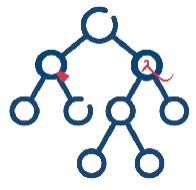
\includegraphics[height=1.0cm]{msca_logo.png}}%
    \end{center}

    \vspace{0.6cm}

    % Main title with Q logos on sides (with clickable links)
    \begin{center}
        \begin{minipage}{0.1\textwidth}
            \centering
            \href{https://quantlet.com}{
\includegraphics[height=1.1cm]{ql_logo.png}}
        \end{minipage}%
        \begin{minipage}{0.78\textwidth}
            \centering
            {\LARGE\bfseries\usebeamercolor[fg]{title}\inserttitle}

            \vspace{0.3cm}

            {\usebeamerfont{subtitle}\usebeamercolor[fg]{title}\insertsubtitle}
        \end{minipage}%
        \begin{minipage}{0.1\textwidth}
            \centering
            \href{https://quantinar.com}{
\includegraphics[height=1.1cm]{qr_logo.png}}
        \end{minipage}
    \end{center}

    \vspace{0.6cm}

    % Authors (left aligned)
    \hspace{0.5cm}{\usebeamerfont{author}\insertauthor}

    \vspace{0.3cm}

    % Institute/Affiliations (left aligned)
    \hspace{0.5cm}\begin{minipage}[t]{0.9\textwidth}
        \raggedright\small\insertinstitute
    \end{minipage}
}

%=============================================================================
% THEOREM ENVIRONMENTS
%=============================================================================
\theoremstyle{definition}
\setbeamertemplate{theorems}[numbered]
\ifdefined\sfmlang
\newtheorem{defn}{Definiție}
\newtheorem{thm}{Teoremă}
\newtheorem{prop}{Propoziție}
\newtheorem{rmk}{Observație}
\else
\newtheorem{defn}{Definition}
\newtheorem{thm}{Theorem}
\newtheorem{prop}{Proposition}
\newtheorem{rmk}{Remark}
\fi

%=============================================================================
% CENTRED MINIPAGE (no extra vertical space)
%=============================================================================
\newenvironment{cminipage}[1]{%
    \par\noindent\hfill\begin{minipage}{#1}\ignorespaces
}{%
    \end{minipage}\hfill\null\par
}

%=============================================================================
% CUSTOM COMMANDS
%=============================================================================
\newcommand{\E}{\mathbb{E}}
\newcommand{\Var}{\text{Var}}
\newcommand{\Cov}{\text{Cov}}
\newcommand{\Corr}{\text{Corr}}
\newcommand{\R}{\mathbb{R}}
\newcommand{\N}{\mathbb{N}}
\newcommand{\Z}{\mathbb{Z}}
\newcommand{\B}{\mathbf{B}}
\newcommand{\imark}{\textcolor{MainBlue}{\textbullet}}
\newcommand{\RMSE}{\text{RMSE}}
\newcommand{\MAE}{\text{MAE}}
\newcommand{\MAPE}{\text{MAPE}}

 se definește
%   \newcommand{\coursename}{Statistics of Financial Markets}      (EN)
%   \newcommand{\coursename}{Statistica piețelor financiare}       (RO)  și  \def\sfmlang{ro}
% Fișierele .tex se află în EN/Courses, EN/Seminars, RO/Cursuri, RO/Seminarii (două niveluri sub rădăcină).
% Deck-urile sînt generate de latex/build_chapterN.py / build_seminarN.py (vezi latex/sfm_build.py).

\documentclass[9pt, aspectratio=169, t]{beamer}
\providecommand{\coursename}{Statistics of Financial Markets}

% Ensure content fits on slides
\setbeamersize{text margin left=8mm, text margin right=8mm}

%=============================================================================
% THEME AND STYLE CONFIGURATION
%=============================================================================
\usetheme{default}
% Using default theme for clean header/footer control

% Color Palette (matching Redispatch PDF)
\definecolor{MainBlue}{RGB}{26, 58, 110}
\definecolor{AccentBlue}{RGB}{26, 58, 110}
\definecolor{IDAred}{RGB}{205, 0, 0}
\definecolor{DarkGray}{RGB}{51, 51, 51}
\definecolor{MediumGray}{RGB}{128, 128, 128}
\definecolor{LightGray}{RGB}{248, 248, 248}
\definecolor{VeryLightGray}{RGB}{235, 235, 235}
\definecolor{KeynoteGray}{RGB}{218, 218, 218}
\definecolor{SectionGray}{RGB}{120, 120, 120}
\definecolor{FooterGray}{RGB}{100, 100, 100}
\definecolor{Crimson}{RGB}{220, 53, 69}
\definecolor{Forest}{RGB}{46, 125, 50}
\definecolor{Amber}{RGB}{181, 133, 63}
\definecolor{Orange}{RGB}{230, 126, 34}
\definecolor{Purple}{RGB}{142, 68, 173}

% Gradient background (exact Keynote 315° gradient: white to RGB 218,218,218)
\setbeamertemplate{background}{%
    \begin{tikzpicture}[remember picture, overlay]
        \shade[shading=axis, shading angle=315,
        top color=white, bottom color=KeynoteGray]
        (current page.south west) rectangle (current page.north east);
    \end{tikzpicture}%
}
% Fallback solid color for compatibility
\setbeamercolor{background canvas}{bg=}

\setbeamercolor{palette primary}{bg=MainBlue, fg=white}
\setbeamercolor{palette secondary}{bg=MainBlue!85, fg=white}
\setbeamercolor{palette tertiary}{bg=MainBlue!70, fg=white}
\setbeamercolor{structure}{fg=MainBlue}
\setbeamercolor{title}{fg=IDAred}
\setbeamercolor{frametitle}{fg=IDAred, bg=}
\setbeamercolor{block title}{bg=MainBlue, fg=white}
\setbeamercolor{block body}{bg=VeryLightGray, fg=DarkGray}
\setbeamercolor{block title alerted}{bg=Crimson, fg=white}
\setbeamercolor{block body alerted}{bg=Crimson!8, fg=DarkGray}
\setbeamercolor{block title example}{bg=Forest, fg=white}
\setbeamercolor{block body example}{bg=Forest!8, fg=DarkGray}
\setbeamercolor{item}{fg=MainBlue}

% Footer colors (override Madrid theme blue)
\setbeamercolor{author in head/foot}{fg=FooterGray, bg=}
\setbeamercolor{title in head/foot}{fg=FooterGray, bg=}
\setbeamercolor{date in head/foot}{fg=FooterGray, bg=}
\setbeamercolor{section in head/foot}{fg=FooterGray, bg=}
\setbeamercolor{subsection in head/foot}{fg=FooterGray, bg=}

% Bullet styles (apply everywhere including blocks)
\setbeamertemplate{itemize item}{\color{MainBlue}$\boxdot$}
\setbeamertemplate{itemize subitem}{\color{MainBlue}$\blacktriangleright$}
\setbeamertemplate{itemize subsubitem}{\color{MainBlue}\tiny$\bullet$}
\setbeamertemplate{itemize/enumerate body begin}{\normalsize}
\setbeamertemplate{itemize/enumerate subbody begin}{\normalsize}

% Item spacing - compact style
\setlength{\leftmargini}{10pt}       % Level 1: minimal indent
\setlength{\leftmarginii}{10pt}      % Level 2: minimal additional indent
% Compact list spacing (zero extra space before/after lists in blocks)
\makeatletter
\def\@listi{\leftmargin\leftmargini \topsep 0pt \parsep 0pt \itemsep 0pt}
\def\@listii{\leftmargin\leftmarginii \topsep 0pt \parsep 0pt \itemsep 0pt}
\makeatother

\setbeamertemplate{navigation symbols}{}

%=============================================================================
% CUSTOM HEADLINE
%=============================================================================
\setbeamertemplate{headline}{%
    \vskip10pt%
    \hbox to \paperwidth{%
        \hskip0.5cm%
        {\small\color{FooterGray}\renewcommand{\hyperlink}[2]{##2}\insertsectionhead}%
        \hfill%
        \textcolor{FooterGray}{\small\insertframenumber}%
        \hskip0.5cm%
    }%
    \vskip4pt%
    {\color{FooterGray}\hrule height 0.4pt}%
}

%=============================================================================
% CUSTOM FOOTER
%=============================================================================
\usepackage{fontawesome5}

\setbeamertemplate{footline}{%
    {\color{FooterGray}\hrule height 0.4pt}%
    \vskip4pt%
    \hbox to \paperwidth{%
        \hskip0.5cm%
        \textcolor{FooterGray}{\small\coursename}%
        \hfill%
        \raisebox{-0.1em}{%
            \begin{tikzpicture}[x=0.08em, y=0.08em, line width=0.4pt]
                \draw[FooterGray] (0,3) -- (1,4) -- (2,3.5) -- (3,5) -- (4,4) -- (5,6) -- (6,5.5) -- (7,4) -- (8,5) -- (9,7) -- (10,6) -- (11,5) -- (12,6.5) -- (13,8) -- (14,7) -- (15,6) -- (16,7.5) -- (17,9) -- (18,8) -- (19,7) -- (20,8.5) -- (21,10) -- (22,9) -- (23,8) -- (24,9.5);
            \end{tikzpicture}%
        }%
        \hskip0.5cm%
    }%
    \vskip6pt%
}

%=============================================================================
% PACKAGES
%=============================================================================
\usepackage[utf8]{inputenc}
\DeclareUnicodeCharacter{03B1}{\ensuremath{\alpha}}
\usepackage[T1]{fontenc}
\usepackage{amsmath, amssymb, amsthm}
\usepackage{mathtools}
\usepackage{bm}
\usepackage{tikz}
\usetikzlibrary{arrows.meta, positioning, shapes, calc, decorations.pathreplacing, shadings}
\usepackage{booktabs}
\usepackage{multirow}
\usepackage{array}
\usepackage{graphicx}
\usepackage{hyperref}
\usepackage{colortbl}
\usepackage{listings}
\lstset{language=Python, basicstyle=\ttfamily\scriptsize, keywordstyle=\color{MainBlue}\bfseries,
  commentstyle=\color{Forest}, stringstyle=\color{Crimson}, breaklines=true,
  frame=none, backgroundcolor=\color{VeryLightGray}, xleftmargin=2mm}
\hypersetup{colorlinks=true, linkcolor=MainBlue, urlcolor=MainBlue}
\graphicspath{{../../logos/}{../../charts/}{../../photos/}}
\usepackage{xcolor}
\hfuzz=2pt  % Suppress tiny overfull warnings (<2pt)
\vfuzz=2pt  % Suppress tiny vertical overfull warnings (<2pt)

%=============================================================================
% QUANTLET COMMANDS
%   \quantlet{<displayed name>}{<url>}       (generic, compatible with the older SFM decks)
%   \sfmquantlet{Ch_05}{SFM_ch5_garch}       -> https://github.com/danpele/SFM/tree/main/Quantlets/Ch_05/SFM_ch5_garch
%   \qlurl{<folder>} is defined per chapter by the generator (Quantlets/Ch_NN/<folder>)
%=============================================================================
\newcommand{\sfmrepo}{https://github.com/danpele/SFM}
\newcommand{\sfmqlbase}{https://github.com/danpele/SFM/tree/main/Quantlets}
\newcommand{\quantlet}[2]{%
    \hfill\href{#2}{%
        \raisebox{-0.15em}{
\includegraphics[height=0.7em]{ql_logo.png}}%
        \textcolor{MainBlue}{\tiny\ #1}%
    }%
}
\newcommand{\sfmquantlet}[2]{\quantlet{\detokenize{#2}}{\sfmqlbase/#1/#2}}

%=============================================================================
% NOTEBOOKS (Google Colab)
%   \colaburl{notebooks/EN/chapter5_seminar_notebook.ipynb} -> the Colab link of a file in the SFM repo
%   \nb: the chapter notebook (each seminar deck redefines it with \renewcommand)
%=============================================================================
\newcommand{\colaburl}[1]{https://colab.research.google.com/github/danpele/SFM/blob/main/#1}
\newcommand{\nb}{https://colab.research.google.com/github/danpele/SFM/tree/main/notebooks/EN}
\newcommand{\nbname}{notebooks/EN}

%=============================================================================
% SLIDE HELPERS (used by the generators; the same as in MFM)
%=============================================================================
% local font size for list bodies (the preamble forces \normalsize)
\newcommand{\itemsize}[1]{\setbeamertemplate{itemize/enumerate body begin}{#1}\setbeamertemplate{itemize/enumerate subbody begin}{#1}}
\newcommand{\intitle}[1]{{\hypersetup{urlcolor=white}#1}}   % white links inside coloured title bars
\newcommand{\imgcap}[1]{{\scriptsize #1}\\[0.5mm]}          % caption under a photo
\newcommand{\imgcredit}[2]{{\tiny\color{FooterGray}\href{#1}{#2}}}   % image credit: source URL, author/licence
\newcommand{\aiprompt}[1]{{\ttfamily\color{MainBlue}#1}}     % a prompt to an AI assistant

%=============================================================================
% SEMINARS: student version by default; the instructor wrapper *_solutions.tex sets \solutionstrue
%=============================================================================
\makeatletter\@ifundefined{ifsolutions}{\expandafter\newif\csname ifsolutions\endcsname}{}\makeatother
\newcommand{\solonly}[1]{\ifsolutions #1\fi}
\newcommand{\propsub}{\ifsolutions\else\framesubtitle{\ifdefined\sfmlang Rezolvarea se discută la seminar\else Solution discussed in class\fi}\fi}

%=============================================================================
% APPENDIX AND CHAPTER LINKS (latex/appendix_links.py writes the calls; it also re-declares these
% macros before \begin{document}, so the decks compile with or without this preamble block)
%=============================================================================
\providecommand{\sfmapplink}[3]{\hypertarget{#2}{}\hyperlink{#1}{\beamergotobutton{#3}}}
\providecommand{\sfmappback}[2]{\begin{tikzpicture}[remember picture,overlay]\node[anchor=south east] at ([xshift=-3mm,yshift=7mm]current page.south east){\hyperlink{#1}{\beamerreturnbutton{#2}}};\end{tikzpicture}}
\providecommand{\sfmchlink}[2]{\href{#1}{#2}}
\providecommand{\sfmchlinkt}[2]{\href{#1}{\usebeamercolor[fg]{frametitle}#2}}

%=============================================================================
% QUANTINAR COMMAND: link către un curs Quantinar (subiecte avansate)
%=============================================================================
\newcommand{\quantinar}[2]{%
    \href{#2}{%
        \raisebox{-0.15em}{
\includegraphics[height=0.8em]{qr_logo.png}}%
        \textcolor{MainBlue}{\scriptsize\ #1}%
    }%
}

%=============================================================================
% CUSTOM TITLE PAGE
%=============================================================================
\defbeamertemplate*{title page}{hybrid}[1][]
{
    \vspace{0.2cm}
    % Logos row - top header (with clickable links)
    \begin{center}
        \href{https://www.ase.ro}{
\includegraphics[height=1.0cm]{ase_logo.png}}\hspace{0.3cm}%
        \href{https://theida.net}{
\includegraphics[height=1.0cm]{ida_logo.png}}\hspace{0.3cm}%
        \href{https://blockchain-research-center.com}{
\includegraphics[height=1.0cm]{brc_logo.png}}\hspace{0.3cm}%
        \href{https://www.ai4efin.ase.ro}{
\includegraphics[height=1.0cm]{ai4efin_logo.png}}\hspace{0.3cm}%
        \href{https://ipe.ro/new}{
\includegraphics[height=1.0cm]{acad_logo.png}}\hspace{0.3cm}%
        \href{https://www.digital-finance-msca.com}{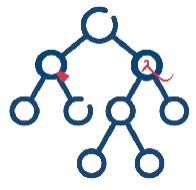
\includegraphics[height=1.0cm]{msca_logo.png}}%
    \end{center}

    \vspace{0.6cm}

    % Main title with Q logos on sides (with clickable links)
    \begin{center}
        \begin{minipage}{0.1\textwidth}
            \centering
            \href{https://quantlet.com}{
\includegraphics[height=1.1cm]{ql_logo.png}}
        \end{minipage}%
        \begin{minipage}{0.78\textwidth}
            \centering
            {\LARGE\bfseries\usebeamercolor[fg]{title}\inserttitle}

            \vspace{0.3cm}

            {\usebeamerfont{subtitle}\usebeamercolor[fg]{title}\insertsubtitle}
        \end{minipage}%
        \begin{minipage}{0.1\textwidth}
            \centering
            \href{https://quantinar.com}{
\includegraphics[height=1.1cm]{qr_logo.png}}
        \end{minipage}
    \end{center}

    \vspace{0.6cm}

    % Authors (left aligned)
    \hspace{0.5cm}{\usebeamerfont{author}\insertauthor}

    \vspace{0.3cm}

    % Institute/Affiliations (left aligned)
    \hspace{0.5cm}\begin{minipage}[t]{0.9\textwidth}
        \raggedright\small\insertinstitute
    \end{minipage}
}

%=============================================================================
% THEOREM ENVIRONMENTS
%=============================================================================
\theoremstyle{definition}
\setbeamertemplate{theorems}[numbered]
\ifdefined\sfmlang
\newtheorem{defn}{Definiție}
\newtheorem{thm}{Teoremă}
\newtheorem{prop}{Propoziție}
\newtheorem{rmk}{Observație}
\else
\newtheorem{defn}{Definition}
\newtheorem{thm}{Theorem}
\newtheorem{prop}{Proposition}
\newtheorem{rmk}{Remark}
\fi

%=============================================================================
% CENTRED MINIPAGE (no extra vertical space)
%=============================================================================
\newenvironment{cminipage}[1]{%
    \par\noindent\hfill\begin{minipage}{#1}\ignorespaces
}{%
    \end{minipage}\hfill\null\par
}

%=============================================================================
% CUSTOM COMMANDS
%=============================================================================
\newcommand{\E}{\mathbb{E}}
\newcommand{\Var}{\text{Var}}
\newcommand{\Cov}{\text{Cov}}
\newcommand{\Corr}{\text{Corr}}
\newcommand{\R}{\mathbb{R}}
\newcommand{\N}{\mathbb{N}}
\newcommand{\Z}{\mathbb{Z}}
\newcommand{\B}{\mathbf{B}}
\newcommand{\imark}{\textcolor{MainBlue}{\textbullet}}
\newcommand{\RMSE}{\text{RMSE}}
\newcommand{\MAE}{\text{MAE}}
\newcommand{\MAPE}{\text{MAPE}}

 se definește
%   \newcommand{\coursename}{Statistics of Financial Markets}      (EN)
%   \newcommand{\coursename}{Statistica piețelor financiare}       (RO)  și  \def\sfmlang{ro}
% Fișierele .tex se află în EN/Courses, EN/Seminars, RO/Cursuri, RO/Seminarii (două niveluri sub rădăcină).
% Deck-urile sînt generate de latex/build_chapterN.py / build_seminarN.py (vezi latex/sfm_build.py).

\documentclass[9pt, aspectratio=169, t]{beamer}
\providecommand{\coursename}{Statistics of Financial Markets}

% Ensure content fits on slides
\setbeamersize{text margin left=8mm, text margin right=8mm}

%=============================================================================
% THEME AND STYLE CONFIGURATION
%=============================================================================
\usetheme{default}
% Using default theme for clean header/footer control

% Color Palette (matching Redispatch PDF)
\definecolor{MainBlue}{RGB}{26, 58, 110}
\definecolor{AccentBlue}{RGB}{26, 58, 110}
\definecolor{IDAred}{RGB}{205, 0, 0}
\definecolor{DarkGray}{RGB}{51, 51, 51}
\definecolor{MediumGray}{RGB}{128, 128, 128}
\definecolor{LightGray}{RGB}{248, 248, 248}
\definecolor{VeryLightGray}{RGB}{235, 235, 235}
\definecolor{KeynoteGray}{RGB}{218, 218, 218}
\definecolor{SectionGray}{RGB}{120, 120, 120}
\definecolor{FooterGray}{RGB}{100, 100, 100}
\definecolor{Crimson}{RGB}{220, 53, 69}
\definecolor{Forest}{RGB}{46, 125, 50}
\definecolor{Amber}{RGB}{181, 133, 63}
\definecolor{Orange}{RGB}{230, 126, 34}
\definecolor{Purple}{RGB}{142, 68, 173}

% Gradient background (exact Keynote 315° gradient: white to RGB 218,218,218)
\setbeamertemplate{background}{%
    \begin{tikzpicture}[remember picture, overlay]
        \shade[shading=axis, shading angle=315,
        top color=white, bottom color=KeynoteGray]
        (current page.south west) rectangle (current page.north east);
    \end{tikzpicture}%
}
% Fallback solid color for compatibility
\setbeamercolor{background canvas}{bg=}

\setbeamercolor{palette primary}{bg=MainBlue, fg=white}
\setbeamercolor{palette secondary}{bg=MainBlue!85, fg=white}
\setbeamercolor{palette tertiary}{bg=MainBlue!70, fg=white}
\setbeamercolor{structure}{fg=MainBlue}
\setbeamercolor{title}{fg=IDAred}
\setbeamercolor{frametitle}{fg=IDAred, bg=}
\setbeamercolor{block title}{bg=MainBlue, fg=white}
\setbeamercolor{block body}{bg=VeryLightGray, fg=DarkGray}
\setbeamercolor{block title alerted}{bg=Crimson, fg=white}
\setbeamercolor{block body alerted}{bg=Crimson!8, fg=DarkGray}
\setbeamercolor{block title example}{bg=Forest, fg=white}
\setbeamercolor{block body example}{bg=Forest!8, fg=DarkGray}
\setbeamercolor{item}{fg=MainBlue}

% Footer colors (override Madrid theme blue)
\setbeamercolor{author in head/foot}{fg=FooterGray, bg=}
\setbeamercolor{title in head/foot}{fg=FooterGray, bg=}
\setbeamercolor{date in head/foot}{fg=FooterGray, bg=}
\setbeamercolor{section in head/foot}{fg=FooterGray, bg=}
\setbeamercolor{subsection in head/foot}{fg=FooterGray, bg=}

% Bullet styles (apply everywhere including blocks)
\setbeamertemplate{itemize item}{\color{MainBlue}$\boxdot$}
\setbeamertemplate{itemize subitem}{\color{MainBlue}$\blacktriangleright$}
\setbeamertemplate{itemize subsubitem}{\color{MainBlue}\tiny$\bullet$}
\setbeamertemplate{itemize/enumerate body begin}{\normalsize}
\setbeamertemplate{itemize/enumerate subbody begin}{\normalsize}

% Item spacing - compact style
\setlength{\leftmargini}{10pt}       % Level 1: minimal indent
\setlength{\leftmarginii}{10pt}      % Level 2: minimal additional indent
% Compact list spacing (zero extra space before/after lists in blocks)
\makeatletter
\def\@listi{\leftmargin\leftmargini \topsep 0pt \parsep 0pt \itemsep 0pt}
\def\@listii{\leftmargin\leftmarginii \topsep 0pt \parsep 0pt \itemsep 0pt}
\makeatother

\setbeamertemplate{navigation symbols}{}

%=============================================================================
% CUSTOM HEADLINE
%=============================================================================
\setbeamertemplate{headline}{%
    \vskip10pt%
    \hbox to \paperwidth{%
        \hskip0.5cm%
        {\small\color{FooterGray}\renewcommand{\hyperlink}[2]{##2}\insertsectionhead}%
        \hfill%
        \textcolor{FooterGray}{\small\insertframenumber}%
        \hskip0.5cm%
    }%
    \vskip4pt%
    {\color{FooterGray}\hrule height 0.4pt}%
}

%=============================================================================
% CUSTOM FOOTER
%=============================================================================
\usepackage{fontawesome5}

\setbeamertemplate{footline}{%
    {\color{FooterGray}\hrule height 0.4pt}%
    \vskip4pt%
    \hbox to \paperwidth{%
        \hskip0.5cm%
        \textcolor{FooterGray}{\small\coursename}%
        \hfill%
        \raisebox{-0.1em}{%
            \begin{tikzpicture}[x=0.08em, y=0.08em, line width=0.4pt]
                \draw[FooterGray] (0,3) -- (1,4) -- (2,3.5) -- (3,5) -- (4,4) -- (5,6) -- (6,5.5) -- (7,4) -- (8,5) -- (9,7) -- (10,6) -- (11,5) -- (12,6.5) -- (13,8) -- (14,7) -- (15,6) -- (16,7.5) -- (17,9) -- (18,8) -- (19,7) -- (20,8.5) -- (21,10) -- (22,9) -- (23,8) -- (24,9.5);
            \end{tikzpicture}%
        }%
        \hskip0.5cm%
    }%
    \vskip6pt%
}

%=============================================================================
% PACKAGES
%=============================================================================
\usepackage[utf8]{inputenc}
\DeclareUnicodeCharacter{03B1}{\ensuremath{\alpha}}
\usepackage[T1]{fontenc}
\usepackage{amsmath, amssymb, amsthm}
\usepackage{mathtools}
\usepackage{bm}
\usepackage{tikz}
\usetikzlibrary{arrows.meta, positioning, shapes, calc, decorations.pathreplacing, shadings}
\usepackage{booktabs}
\usepackage{multirow}
\usepackage{array}
\usepackage{graphicx}
\usepackage{hyperref}
\usepackage{colortbl}
\usepackage{listings}
\lstset{language=Python, basicstyle=\ttfamily\scriptsize, keywordstyle=\color{MainBlue}\bfseries,
  commentstyle=\color{Forest}, stringstyle=\color{Crimson}, breaklines=true,
  frame=none, backgroundcolor=\color{VeryLightGray}, xleftmargin=2mm}
\hypersetup{colorlinks=true, linkcolor=MainBlue, urlcolor=MainBlue}
\graphicspath{{../../logos/}{../../charts/}{../../photos/}}
\usepackage{xcolor}
\hfuzz=2pt  % Suppress tiny overfull warnings (<2pt)
\vfuzz=2pt  % Suppress tiny vertical overfull warnings (<2pt)

%=============================================================================
% QUANTLET COMMANDS
%   \quantlet{<displayed name>}{<url>}       (generic, compatible with the older SFM decks)
%   \sfmquantlet{Ch_05}{SFM_ch5_garch}       -> https://github.com/danpele/SFM/tree/main/Quantlets/Ch_05/SFM_ch5_garch
%   \qlurl{<folder>} is defined per chapter by the generator (Quantlets/Ch_NN/<folder>)
%=============================================================================
\newcommand{\sfmrepo}{https://github.com/danpele/SFM}
\newcommand{\sfmqlbase}{https://github.com/danpele/SFM/tree/main/Quantlets}
\newcommand{\quantlet}[2]{%
    \hfill\href{#2}{%
        \raisebox{-0.15em}{
\includegraphics[height=0.7em]{ql_logo.png}}%
        \textcolor{MainBlue}{\tiny\ #1}%
    }%
}
\newcommand{\sfmquantlet}[2]{\quantlet{\detokenize{#2}}{\sfmqlbase/#1/#2}}

%=============================================================================
% NOTEBOOKS (Google Colab)
%   \colaburl{notebooks/EN/chapter5_seminar_notebook.ipynb} -> the Colab link of a file in the SFM repo
%   \nb: the chapter notebook (each seminar deck redefines it with \renewcommand)
%=============================================================================
\newcommand{\colaburl}[1]{https://colab.research.google.com/github/danpele/SFM/blob/main/#1}
\newcommand{\nb}{https://colab.research.google.com/github/danpele/SFM/tree/main/notebooks/EN}
\newcommand{\nbname}{notebooks/EN}

%=============================================================================
% SLIDE HELPERS (used by the generators; the same as in MFM)
%=============================================================================
% local font size for list bodies (the preamble forces \normalsize)
\newcommand{\itemsize}[1]{\setbeamertemplate{itemize/enumerate body begin}{#1}\setbeamertemplate{itemize/enumerate subbody begin}{#1}}
\newcommand{\intitle}[1]{{\hypersetup{urlcolor=white}#1}}   % white links inside coloured title bars
\newcommand{\imgcap}[1]{{\scriptsize #1}\\[0.5mm]}          % caption under a photo
\newcommand{\imgcredit}[2]{{\tiny\color{FooterGray}\href{#1}{#2}}}   % image credit: source URL, author/licence
\newcommand{\aiprompt}[1]{{\ttfamily\color{MainBlue}#1}}     % a prompt to an AI assistant

%=============================================================================
% SEMINARS: student version by default; the instructor wrapper *_solutions.tex sets \solutionstrue
%=============================================================================
\makeatletter\@ifundefined{ifsolutions}{\expandafter\newif\csname ifsolutions\endcsname}{}\makeatother
\newcommand{\solonly}[1]{\ifsolutions #1\fi}
\newcommand{\propsub}{\ifsolutions\else\framesubtitle{\ifdefined\sfmlang Rezolvarea se discută la seminar\else Solution discussed in class\fi}\fi}

%=============================================================================
% APPENDIX AND CHAPTER LINKS (latex/appendix_links.py writes the calls; it also re-declares these
% macros before \begin{document}, so the decks compile with or without this preamble block)
%=============================================================================
\providecommand{\sfmapplink}[3]{\hypertarget{#2}{}\hyperlink{#1}{\beamergotobutton{#3}}}
\providecommand{\sfmappback}[2]{\begin{tikzpicture}[remember picture,overlay]\node[anchor=south east] at ([xshift=-3mm,yshift=7mm]current page.south east){\hyperlink{#1}{\beamerreturnbutton{#2}}};\end{tikzpicture}}
\providecommand{\sfmchlink}[2]{\href{#1}{#2}}
\providecommand{\sfmchlinkt}[2]{\href{#1}{\usebeamercolor[fg]{frametitle}#2}}

%=============================================================================
% QUANTINAR COMMAND: link către un curs Quantinar (subiecte avansate)
%=============================================================================
\newcommand{\quantinar}[2]{%
    \href{#2}{%
        \raisebox{-0.15em}{
\includegraphics[height=0.8em]{qr_logo.png}}%
        \textcolor{MainBlue}{\scriptsize\ #1}%
    }%
}

%=============================================================================
% CUSTOM TITLE PAGE
%=============================================================================
\defbeamertemplate*{title page}{hybrid}[1][]
{
    \vspace{0.2cm}
    % Logos row - top header (with clickable links)
    \begin{center}
        \href{https://www.ase.ro}{
\includegraphics[height=1.0cm]{ase_logo.png}}\hspace{0.3cm}%
        \href{https://theida.net}{
\includegraphics[height=1.0cm]{ida_logo.png}}\hspace{0.3cm}%
        \href{https://blockchain-research-center.com}{
\includegraphics[height=1.0cm]{brc_logo.png}}\hspace{0.3cm}%
        \href{https://www.ai4efin.ase.ro}{
\includegraphics[height=1.0cm]{ai4efin_logo.png}}\hspace{0.3cm}%
        \href{https://ipe.ro/new}{
\includegraphics[height=1.0cm]{acad_logo.png}}\hspace{0.3cm}%
        \href{https://www.digital-finance-msca.com}{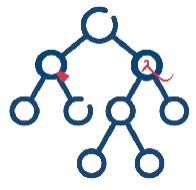
\includegraphics[height=1.0cm]{msca_logo.png}}%
    \end{center}

    \vspace{0.6cm}

    % Main title with Q logos on sides (with clickable links)
    \begin{center}
        \begin{minipage}{0.1\textwidth}
            \centering
            \href{https://quantlet.com}{
\includegraphics[height=1.1cm]{ql_logo.png}}
        \end{minipage}%
        \begin{minipage}{0.78\textwidth}
            \centering
            {\LARGE\bfseries\usebeamercolor[fg]{title}\inserttitle}

            \vspace{0.3cm}

            {\usebeamerfont{subtitle}\usebeamercolor[fg]{title}\insertsubtitle}
        \end{minipage}%
        \begin{minipage}{0.1\textwidth}
            \centering
            \href{https://quantinar.com}{
\includegraphics[height=1.1cm]{qr_logo.png}}
        \end{minipage}
    \end{center}

    \vspace{0.6cm}

    % Authors (left aligned)
    \hspace{0.5cm}{\usebeamerfont{author}\insertauthor}

    \vspace{0.3cm}

    % Institute/Affiliations (left aligned)
    \hspace{0.5cm}\begin{minipage}[t]{0.9\textwidth}
        \raggedright\small\insertinstitute
    \end{minipage}
}

%=============================================================================
% THEOREM ENVIRONMENTS
%=============================================================================
\theoremstyle{definition}
\setbeamertemplate{theorems}[numbered]
\ifdefined\sfmlang
\newtheorem{defn}{Definiție}
\newtheorem{thm}{Teoremă}
\newtheorem{prop}{Propoziție}
\newtheorem{rmk}{Observație}
\else
\newtheorem{defn}{Definition}
\newtheorem{thm}{Theorem}
\newtheorem{prop}{Proposition}
\newtheorem{rmk}{Remark}
\fi

%=============================================================================
% CENTRED MINIPAGE (no extra vertical space)
%=============================================================================
\newenvironment{cminipage}[1]{%
    \par\noindent\hfill\begin{minipage}{#1}\ignorespaces
}{%
    \end{minipage}\hfill\null\par
}

%=============================================================================
% CUSTOM COMMANDS
%=============================================================================
\newcommand{\E}{\mathbb{E}}
\newcommand{\Var}{\text{Var}}
\newcommand{\Cov}{\text{Cov}}
\newcommand{\Corr}{\text{Corr}}
\newcommand{\R}{\mathbb{R}}
\newcommand{\N}{\mathbb{N}}
\newcommand{\Z}{\mathbb{Z}}
\newcommand{\B}{\mathbf{B}}
\newcommand{\imark}{\textcolor{MainBlue}{\textbullet}}
\newcommand{\RMSE}{\text{RMSE}}
\newcommand{\MAE}{\text{MAE}}
\newcommand{\MAPE}{\text{MAPE}}



\newcommand{\qlurl}[1]{https://github.com/danpele/SFM/tree/main/Quantlets/Ch_06/#1}
\renewcommand{\nb}{\colaburl{notebooks/EN/chapter6_seminar_notebook.ipynb}}
\renewcommand{\nbname}{chapter6\_seminar\_notebook.ipynb}
% left column: full width in the student version, narrower next to the solution
\newcommand{\taskw}{\ifsolutions 0.47\textwidth\else 0.96\textwidth\fi}
\newcommand{\solw}{\ifsolutions 0.49\textwidth\else 0pt\fi}

% Clickable citations (DOIs verified via Crossref)

\newcommand{\refFHH}{\href{https://doi.org/10.1007/978-3-030-13751-9}{Franke, Härdle \& Hafner (2019)}}
\newcommand{\refFHHex}{\href{https://doi.org/10.1007/978-3-642-33929-5}{Borak, Härdle \& López-Cabrera (2013)}}
\newcommand{\refTsay}{\href{https://doi.org/10.1002/9780470644560}{Tsay (2010)}}
\newcommand{\refBox}{\href{https://doi.org/10.1080/01621459.1976.10480949}{Box (1976)}}
\newcommand{\refAkaike}{\href{https://doi.org/10.1109/TAC.1974.1100705}{Akaike (1974)}}
\newcommand{\refSchwarz}{\href{https://doi.org/10.1214/aos/1176344136}{Schwarz (1978)}}
\newcommand{\refKL}{\href{https://doi.org/10.1214/aoms/1177729694}{Kullback \& Leibler (1951)}}
\newcommand{\refBA}{\href{https://doi.org/10.1177/0049124104268644}{Burnham \& Anderson (2004)}}
\newcommand{\refBAbook}{\href{https://doi.org/10.1007/b97636}{Burnham \& Anderson (2002)}}
\newcommand{\refStone}{\href{https://doi.org/10.1111/j.2517-6161.1977.tb01603.x}{Stone (1977)}}
\newcommand{\refHT}{\href{https://doi.org/10.1093/biomet/76.2.297}{Hurvich \& Tsai (1989)}}
\newcommand{\refWilks}{\href{https://doi.org/10.1214/aoms/1177732360}{Wilks (1938)}}
\newcommand{\refSL}{\href{https://doi.org/10.1080/01621459.1987.10478472}{Self \& Liang (1987)}}
\newcommand{\refVuong}{\href{https://doi.org/10.2307/1912557}{Vuong (1989)}}
\newcommand{\refPearson}{\href{https://doi.org/10.1080/14786440009463897}{Pearson (1900)}}
\newcommand{\refSmirnov}{\href{https://doi.org/10.1214/aoms/1177730256}{Smirnov (1948)}}
\newcommand{\refLilliefors}{\href{https://doi.org/10.1080/01621459.1967.10482916}{Lilliefors (1967)}}
\newcommand{\refAD}{\href{https://doi.org/10.1214/aoms/1177729437}{Anderson \& Darling (1952)}}
\newcommand{\refADb}{\href{https://doi.org/10.1080/01621459.1954.10501232}{Anderson \& Darling (1954)}}
\newcommand{\refCramer}{\href{https://doi.org/10.1080/03461238.1928.10416862}{Cramér (1928)}}
\newcommand{\refStephens}{\href{https://doi.org/10.1080/01621459.1974.10480196}{Stephens (1974)}}
\newcommand{\refSGQ}{\href{https://doi.org/10.1007/BF02613687}{Stute et al.\ (1993)}}
\newcommand{\refHansen}{\href{https://doi.org/10.2307/2527081}{Hansen (1994)}}
\newcommand{\refNelson}{\href{https://doi.org/10.2307/2938260}{Nelson (1991)}}
\newcommand{\refKon}{\href{https://doi.org/10.1111/j.1540-6261.1984.tb03865.x}{Kon (1984)}}
\newcommand{\refBN}{\href{https://doi.org/10.1111/1467-9469.00045}{Barndorff-Nielsen (1997)}}
\newcommand{\refEK}{\href{https://doi.org/10.2307/3318481}{Eberlein \& Keller (1995)}}
\newcommand{\refKupiec}{\href{https://doi.org/10.3905/jod.1995.407942}{Kupiec (1995)}}
\newcommand{\refGR}{\href{https://doi.org/10.1198/016214506000001437}{Gneiting \& Raftery (2007)}}
\newcommand{\refAG}{\href{https://doi.org/10.1198/073500106000000332}{Amisano \& Giacomini (2007)}}
\newcommand{\refDPD}{\href{https://doi.org/10.1016/j.jeconom.2011.04.001}{Diks, Panchenko \& van Dijk (2011)}}
\newcommand{\refHoeting}{\href{https://doi.org/10.1214/ss/1009212519}{Hoeting et al.\ (1999)}}
\newcommand{\refDanielsson}{\href{https://doi.org/10.1016/j.jfs.2016.02.002}{Danielsson et al.\ (2016)}}
\newcommand{\refKerkhof}{\href{https://doi.org/10.1016/j.jbankfin.2009.07.025}{Kerkhof, Melenberg \& Schumacher (2010)}}
\newcommand{\refCont}{\href{https://doi.org/10.1080/713665670}{Cont (2001)}}
\newcommand{\refPeleA}{\href{https://doi.org/10.3390/e19050226}{Pele, Lazar \& Dufour (2017)}}
\newcommand{\refPeleB}{\href{https://doi.org/10.3390/e21121204}{Pele, Lazar \& Mazurencu-Marinescu-Pele (2019)}}
\newcommand{\refWang}{\href{https://doi.org/10.1038/s41586-023-06221-2}{Wang et al.\ (2023)}}

\title[Statistics of Financial Markets]{Statistics of Financial Markets}
\subtitle{Seminar 6: Model selection and risk management\ifsolutions\ (instructor version)\fi}
\author[D.T. Pele]{Daniel Traian PELE}
\institute{Bucharest University of Economic Studies\\
IDA Institute Digital Assets\\
Blockchain Research Center\\
AI4EFin Artificial Intelligence for Energy Finance\\
Romanian Academy, Institute for Economic Forecasting\\
MSCA Digital Finance}
\date{}

%=============================================================================
\providecommand{\sfmapplink}[3]{\hypertarget{#2}{}\hyperlink{#1}{\beamergotobutton{#3}}}  % APPLINKS-MACROS
\providecommand{\sfmappback}[2]{\begin{tikzpicture}[remember picture,overlay]\node[anchor=south east] at ([xshift=-3mm,yshift=7mm]current page.south east){\hyperlink{#1}{\beamerreturnbutton{#2}}};\end{tikzpicture}}  % APPLINKS-MACROS
\providecommand{\sfmchlink}[2]{\href{#1}{#2}}  % APPLINKS-MACROS
\providecommand{\sfmchlinkt}[2]{\href{#1}{\usebeamercolor[fg]{frametitle}#2}}  % APPLINKS-MACROS
\begin{document}
%=============================================================================

{
\setbeamertemplate{headline}{}
\setbeamertemplate{footline}{}
\begin{frame}[noframenumbering]
    \titlepage
\end{frame}
}
% BEGIN-ACRONYMS (generat de latex/acronyms.py; nu editati manual)
\begin{frame}{Acronyms used in this material}
\setbeamertemplate{itemize/enumerate body begin}{\tiny}
\begin{columns}[T]
\begin{column}{0.49\textwidth}
\begin{itemize}\setlength{\itemsep}{0pt}
    \item \textbf{AD}: Anderson–Darling (test)
    \item \textbf{AI}: Artificial Intelligence
    \item \textbf{AIC}: Akaike Information Criterion
    \item \textbf{BET}: Bucharest Exchange Trading (index)
    \item \textbf{BIC}: Bayesian Information Criterion
    \item \textbf{EDF}: Empirical Distribution Function
    \item \textbf{EODHD}: EOD Historical Data (market-data provider)
    \item \textbf{ES}: Expected Shortfall
    \item \textbf{GED}: Generalised Error Distribution
    \item \textbf{KS}: Kolmogorov–Smirnov (test)
    \item \textbf{LR}: Likelihood Ratio
    \item \textbf{ML}: Maximum Likelihood
    \item \textbf{NIG}: Normal Inverse Gaussian (distribution)
\end{itemize}
\end{column}
\begin{column}{0.49\textwidth}
\begin{itemize}\setlength{\itemsep}{0pt}
    \item \textbf{QQ}: Quantile–Quantile (plot)
\end{itemize}
\end{column}
\end{columns}
\end{frame}
% END-ACRONYMS

\begin{frame}{Today's Question and Route}
\itemsize{\small}
\begin{itemize}
    \item \textbf{Question}: among several candidate distributions for daily returns, which one should we choose, and how do we know it is good enough for VaR 1\%?
    \begin{itemize}
        \item this seminar comes \textbf{before} Lecture 6: the section ``What You Need for Today'' gives every definition the tasks use
    \end{itemize}
    \item Route
    \begin{itemize}
        \item Part A: AIC, BIC, Akaike weights, likelihood-ratio tests, a KS test and VaR exceedances on paper
        \item Part B: model choice on BET, S\&P 500, DAX, Bitcoin and Banca Transilvania, each with an interpretation question
        \item Part C: an open question for a project and an AI answer to audit
    \end{itemize}
    \item Notebook for today: \href{\nb}{open the seminar notebook in Google Colab}; each task names its notebook section
    \item Nothing is handed in: the seminar is for practice; the solutions of [Proposed] tasks are discussed in class
\end{itemize}
\end{frame}

\begin{frame}{Exercise Map}
\itemsize{\small}
\begin{center}
\footnotesize
\begin{tabular}{>{\raggedright\arraybackslash}p{1.1cm}>{\raggedright\arraybackslash}p{7.5cm}>{\raggedright\arraybackslash}p{1.9cm}>{\raggedright\arraybackslash}p{1.4cm}}
\toprule
\textbf{Task} & \textbf{Question} & \textbf{Type} & \textbf{Model} \\
\midrule
A1, A2 & which model has the lowest AIC and BIC, and how strong is the evidence? & Solved, Proposed & A1 \\
A3, A4 & is the larger of two nested models significantly better? & Solved, Proposed & A3 \\
A5, A6 & does a small sample pass a KS test, with known and with estimated parameters? & Solved, Proposed & A5 \\
A7, A8 & VaR 1\% under two models; are the exceedances too many or too few? & Solved, Proposed & A7 \\
B1, B2 & which distribution fits BET, DAX and Bitcoin returns best? & Solved, Proposed & B1 \\
B3, B4 & do the best models pass a goodness-of-fit test? are two TLV days data errors? & Solved, Proposed & B3 \\
B5, B6 & which model gets VaR 1\% right out of sample? & Solved, Proposed & B5 \\
C1, C2 & does the best model change over time? what is wrong in an AI answer? & Proposed & B1, A3 \\
\bottomrule
\end{tabular}
\end{center}
\begin{itemize}
    \item \textbf{[Solved]}: full solution in the slides and in the notebook, a model to follow; \textbf{[Proposed]}: you solve it, following the model
\end{itemize}
\end{frame}

\begin{frame}{Data Used}
\itemsize{\small}
\begin{center}
\footnotesize
\begin{tabular}{llll}
\toprule
\textbf{Series} & \textbf{Source} & \textbf{Price used} & \textbf{Period} \\
\midrule
BET, S\&P 500, DAX & EODHD & close & 2000--2026 \\
Bitcoin & EODHD & close, 7 days a week & 2014--2026 \\
Banca Transilvania (TLV) & EODHD & adjusted close & 2010--2026 \\
\bottomrule
\end{tabular}
\end{center}
\begin{itemize}
    \item Daily log returns in \%: $r_t = 100\,(\ln P_t - \ln P_{t-1})$; weekends and repeated holiday closes are dropped (except Bitcoin)
    \item Six candidate models: Normal, Student-t, skewed-t, GED, two-component Normal mixture, NIG
    \item In the notebook: \texttt{returns('bet')}, \texttt{fit\_model('NIG', x)}; no account or key is needed
\end{itemize}
\end{frame}


%=============================================================================
\section{What You Need for Today}
%=============================================================================

\begin{frame}{What You Need for Today (1/5): Likelihood and the Candidates}
\itemsize{\small}
\begin{itemize}
    \item Returns $r_1, \dots, r_n$ i.i.d.\ (independent, identically distributed) with density $f(r; \theta)$
    \begin{itemize}
        \item log-likelihood $\ell(\theta) = \sum_t \ln f(r_t; \theta)$; the ML (maximum likelihood) estimate $\hat\theta$ maximises it
        \item Normal: $\ell(\hat\theta) = -\frac{n}{2}[\ln(2\pi\hat\sigma^2) + 1]$ with $\hat\sigma^2 = \frac{1}{n}\sum_t (r_t - \bar r)^2$
    \end{itemize}
    \item Candidates and their number of parameters $k$
    \begin{itemize}
        \item Normal (2); Student-t (3: $\nu$, location, scale); skewed-t (4: adds the skewness $\lambda$, $\lambda = 0$ gives the Student-t)
        \item GED, generalised error distribution (3: shape $\beta$, $\beta = 2$ gives the Normal law); Normal mixture of two components (5); NIG, normal inverse Gaussian (4)
    \end{itemize}
    \item The heavier the tails of the data, the more the Normal model loses in $\ell$
\end{itemize}
\end{frame}

\begin{frame}{What You Need for Today (2/5): AIC, BIC, Akaike Weights}
\itemsize{\small}
\begin{itemize}
    \item $\mathrm{AIC} = -2\ell(\hat\theta) + 2k$ (Akaike information criterion); $\mathrm{BIC} = -2\ell(\hat\theta) + k\ln n$ (Bayesian information criterion)
    \begin{itemize}
        \item lower is better; only differences on the same data matter; BIC penalises parameters more when $\ln n > 2$, i.e.\ $n > 7$
    \end{itemize}
    \item $\Delta_i = \mathrm{AIC}_i - \min_j \mathrm{AIC}_j$; Akaike weight $w_i = e^{-\Delta_i/2}/\sum_j e^{-\Delta_j/2}$
    \begin{itemize}
        \item rules of thumb \refBA: $\Delta \le 2$ substantial support; $4$--$7$ considerably less; $> 10$ essentially none
    \end{itemize}
    \item AIC is not a test: there is no $p$-value and no ``significance''
\end{itemize}
\end{frame}

\begin{frame}{What You Need for Today (3/5): the Likelihood-Ratio Test}
\itemsize{\small}
\begin{itemize}
    \item Model 0 is \textbf{nested} in model 1 if it is model 1 with some parameters fixed (Student-t = skewed-t with $\lambda = 0$)
    \begin{itemize}
        \item $LR = 2[\ell_1(\hat\theta_1) - \ell_0(\hat\theta_0)] \approx \chi^2(k_1 - k_0)$ under $H_0$ (Wilks)
        \item 5\% critical values: $\chi^2_{0.95}(1) = 3.84$, $\chi^2_{0.95}(2) = 5.99$
    \end{itemize}
    \item \textbf{Boundary}: Normal inside Student-t means $1/\nu = 0$, the edge of the parameter space
    \begin{itemize}
        \item then $LR$ follows a 50:50 mixture of 0 and $\chi^2(1)$ \refSL: 5\% critical value $2.71$, $p$-value = half of the $\chi^2(1)$ one
    \end{itemize}
    \item Non-nested pairs (Student-t vs GED): no LR test; use AIC or the Vuong test
\end{itemize}
\end{frame}

\begin{frame}{What You Need for Today (4/5): Goodness-of-Fit Tests}
\itemsize{\small}
\begin{itemize}
    \item EDF (empirical distribution function) $F_n(x) = \frac{1}{n}\#\{t: r_t \le x\}$; model distribution function $F$
    \begin{itemize}
        \item \textbf{KS} (Kolmogorov--Smirnov): $D_n = \max_i \max\{i/n - u_{(i)},\ u_{(i)} - (i-1)/n\}$ with $u_{(i)} = F(r_{(i)})$ on the sorted data
        \item \textbf{CvM} (Cramér--von Mises) and \textbf{AD} (Anderson--Darling) integrate the squared gap; AD weights it by $1/[F(1-F)]$: it looks at the tails
    \end{itemize}
    \item Critical values of KS at 5\%
    \begin{itemize}
        \item $F$ fully known: $n = 5$: $0.563$; $n = 6$: $0.519$; large $n$: $1.358/\sqrt{n}$
        \item mean and variance estimated from the same data (Lilliefors): $n = 5$: $0.354$; $n = 6$: $0.333$; other models: parametric bootstrap
    \end{itemize}
    \item A QQ plot puts the sorted data against the model quantiles $F^{-1}((i - 0.5)/n)$: tails that bend away from the line are wrong
\end{itemize}
\end{frame}

\begin{frame}{What You Need for Today (5/5): VaR, Exceedances, Out of Sample}
\itemsize{\footnotesize}
\begin{itemize}
    \item $\mathrm{VaR}_{1\%} = -q_{1\%}$, the daily loss exceeded with probability 1\%; Normal: $\mathrm{VaR}_{1\%} = -(\mu - 2.326\sigma)$
    \begin{itemize}
        \item ES 2.5\% (expected shortfall): the average loss beyond $q_{2.5\%}$; Normal: $-\mu + \sigma\varphi(z_{0.025})/0.025$
    \end{itemize}
    \item \textbf{Exceedance}: a day with $r_t < -\mathrm{VaR}$; under a correct model $x \sim \mathrm{Binomial}(n, 0.01)$
    \begin{itemize}
        \item Kupiec test: $LR_{uc} = -2[\ell_0 - \ell_1]$, $\ell_0 = (n - x)\ln 0.99 + x\ln 0.01$, $\ell_1 = (n - x)\ln(1 - \hat p) + x\ln\hat p$, $\hat p = x/n$; compare with $\chi^2(1)$
    \end{itemize}
    \item \textbf{Out of sample}: fit until a date, evaluate afterwards
    \begin{itemize}
        \item log score: mean of $\ln f(r_t; \hat\theta)$ on the test days (higher is better); pinball loss of the 1\% quantile $q$: mean of $(0.01 - \mathbf{1}\{r_t < q\})(r_t - q)$ (lower is better)
    \end{itemize}
\end{itemize}
\end{frame}


%=============================================================================
\section{Part A: Computations on Paper}
%=============================================================================

\begin{frame}{A1: Four Models for the S\&P 500 [Solved]}
\itemsize{\scriptsize}
\begin{columns}[T]
\begin{column}{0.47\textwidth}
\begin{block}{Task}
\begin{itemize}
    \item S\&P 500, the last $n = 1000$ trading days (2022--2026); maximised log-likelihoods:
    \item Normal: $\ell = -1400.9$, $k = 2$
    \item Student-t: $\ell = -1314.7$, $k = 3$
    \item skewed-t: $\ell = -1313.8$, $k = 4$
    \item GED: $\ell = -1322.6$, $k = 3$
    \item 1. Compute AIC and BIC ($\ln 1000 = 6.908$) of each model.
    \item 2. Compute $\Delta$AIC and the Akaike weights.
    \item 3. Say which model each criterion selects and how strong the evidence is.
    \item Report: a table with four rows and two sentences.
\end{itemize}
\end{block}
\end{column}
\begin{column}{0.49\textwidth}
\begin{exampleblock}{Solution}
\begin{itemize}
    \item 1. AIC: Normal $2805.8$, Student-t $2635.4$, skewed-t $2635.6$, GED $2651.2$; BIC: $2815.6$, $2650.1$, $2655.2$, $2665.9$
    \item 2. $\Delta$AIC: $170.4$, $0.0$, $0.2$, $15.8$; $e^{-\Delta/2}$: $0.000$, $1.000$, $0.905$, $0.000$; weights $0.000$, $0.525$, $0.475$, $0.000$
    \item 3. AIC: Student-t and skewed-t tied ($\Delta = 0.2$); BIC: Student-t, by $5.1$ points; Normal and GED have no support.
\end{itemize}
\end{exampleblock}
\end{column}
\end{columns}
\end{frame}

\begin{frame}{A2: Four Models for Bitcoin [Proposed]}
\propsub
\itemsize{\scriptsize}
\begin{columns}[T]
\begin{column}{\taskw}
\begin{block}{Task}
\begin{itemize}
    \item Bitcoin, the last $n = 1000$ days (2023--2026); maximised log-likelihoods: Model: A1.
    \item Normal: $\ell = -2328.0$, $k = 2$
    \item Student-t: $\ell = -2262.0$, $k = 3$
    \item NIG: $\ell = -2258.4$, $k = 4$
    \item Normal mixture: $\ell = -2262.3$, $k = 5$
    \item 1. Compute AIC, BIC, $\Delta$AIC and the Akaike weights.
    \item 2. Say whether AIC and BIC select the same model.
    \item 3. Explain why the Normal mixture, with the most parameters, does not win.
    \item Report: a table with four rows and two sentences.
\end{itemize}
\end{block}
\end{column}
\begin{column}{\solw}
\solonly{%
\begin{exampleblock}{Solution}
\begin{itemize}
    \item 1. AIC: $4660.0$, $4530.0$, $4524.8$, $4534.6$; BIC: $4669.8$, $4544.7$, $4544.4$, $4559.1$; weights $0.000$, $0.069$, $0.924$, $0.007$
    \item 2. AIC: NIG ($\Delta$ of the Student-t $5.2$); BIC: NIG and Student-t almost tied ($\Delta$BIC $0.3$).
    \item 3. Its $\ell$ is no higher than that of the Student-t, and it pays for two more parameters: a Normal mixture has Normal (thin) tails.
\end{itemize}
\end{exampleblock}
}
\end{column}
\end{columns}
\end{frame}

\begin{frame}{A3: Is Skewness Needed? Is the Normal Law Enough? [Solved]}
\itemsize{\scriptsize}
\begin{columns}[T]
\begin{column}{0.47\textwidth}
\begin{block}{Task}
\begin{itemize}
    \item Use the log-likelihoods of A1 (S\&P 500, $n = 1000$).
    \item 1. Test the Student-t ($H_0$: $\lambda = 0$) against the skewed-t with a likelihood-ratio test at 5\%.
    \item 2. Test the Normal law ($H_0$: $\beta = 2$) against the GED.
    \item 3. Compare the LR decision of step 1 with the AIC verdict of A1.
    \item Report: two $LR$ values, two decisions and one sentence.
\end{itemize}
\end{block}
\end{column}
\begin{column}{0.49\textwidth}
\begin{exampleblock}{Solution}
\begin{itemize}
    \item 1. $LR = 2(-1313.8 - (-1314.7)) = 1.8 < 3.84$, $p = 0.18$: do not reject $\lambda = 0$
    \item 2. $LR = 2(-1322.6 - (-1400.9)) = 156.6$, $p <0.001$: reject the Normal law
    \item 3. Consistent: AIC finds the two t-models tied; the LR test finds no significant gain from $\lambda$. For nested pairs, AIC prefers the larger model exactly when $LR > 2$ per extra parameter.
\end{itemize}
\end{exampleblock}
\end{column}
\end{columns}
\end{frame}

\begin{frame}{A4: A Test on the Boundary [Proposed]}
\propsub
\itemsize{\scriptsize}
\begin{columns}[T]
\begin{column}{\taskw}
\begin{block}{Task}
\begin{itemize}
    \item Use the log-likelihoods of A2 (Bitcoin, $n = 1000$). Model: A3.
    \item 1. Compute $LR$ for the Normal law inside the Student-t.
    \item 2. Explain why the null law is not $\chi^2(1)$, and give the correct 5\% critical value.
    \item 3. Say whether an LR test can compare the Student-t with the NIG.
    \item Report: one $LR$ value, one critical value and two sentences.
\end{itemize}
\end{block}
\end{column}
\begin{column}{\solw}
\solonly{%
\begin{exampleblock}{Solution}
\begin{itemize}
    \item 1. $LR = 2(-2262.0 - (-2328.0)) = 132.0$
    \item 2. $H_0$ is $1/\nu = 0$, on the edge of $1/\nu \ge 0$: the law is a 50:50 mixture of 0 and $\chi^2(1)$, critical value $\chi^2_{0.90}(1) = 2.71$; reject the Normal law either way.
    \item 3. No: neither model is a special case of the other; use AIC or the Vuong test.
\end{itemize}
\end{exampleblock}
}
\end{column}
\end{columns}
\end{frame}

\begin{frame}{A5: KS on Five Returns [Solved]}
\itemsize{\scriptsize}
\begin{columns}[T]
\begin{column}{0.47\textwidth}
\begin{block}{Task}
\begin{itemize}
    \item Daily returns (\%): $-2.1$, $-0.4$, $0.3$, $0.9$, $1.6$.
    \item 1. Compute $D_5$ against $N(0, 1)$ and compare it with the 5\% critical value $0.563$.
    \item 2. Estimate $\hat\mu$ and $\hat\sigma$ (divisor $n$), compute $D_5$ against $N(\hat\mu, \hat\sigma^2)$ and compare it with the Lilliefors value $0.354$.
    \item 3. Explain why the Lilliefors critical value is smaller.
    \item Report: two values of $D_5$, two decisions, one sentence.
\end{itemize}
\end{block}
\end{column}
\begin{column}{0.49\textwidth}
\begin{exampleblock}{Solution}
\begin{itemize}
    \item 1. $u_{(i)} = \Phi(r_{(i)})$: $0.018$, $0.345$, $0.618$, $0.816$, $0.945$; the largest gap $D_5 = 0.218 < 0.563$: do not reject
    \item 2. $\hat\mu = 0.060$, $\hat\sigma = 1.266$; $z_{(i)}$: $-1.71$, $-0.36$, $0.19$, $0.66$, $1.22$; $u_{(i)}$: $0.044$, $0.358$, $0.575$, $0.747$, $0.888$; $D_5 = 0.175 < 0.354$: do not reject
    \item 3. The fitted $F$ is pulled towards the data, so $D_n$ is smaller under $H_0$; the critical value must be smaller too.
\end{itemize}
\end{exampleblock}
\end{column}
\end{columns}
\end{frame}

\begin{frame}{A6: KS with One Large Loss [Proposed]}
\propsub
\itemsize{\scriptsize}
\begin{columns}[T]
\begin{column}{\taskw}
\begin{block}{Task}
\begin{itemize}
    \item Daily returns (\%): $-3.0$, $-0.6$, $-0.2$, $0.1$, $0.5$, $1.0$. Model: A5.
    \item 1. Compute $D_6$ against $N(0, 1)$; the 5\% critical value is $0.519$.
    \item 2. Compute $D_6$ against $N(\hat\mu, \hat\sigma^2)$; the Lilliefors value is $0.333$.
    \item 3. The $-3\%$ day has $\Phi(-3) = 0.001$; explain why KS hardly reacts to it, while AD would.
    \item Report: two values of $D_6$, two decisions, one sentence.
\end{itemize}
\end{block}
\end{column}
\begin{column}{\solw}
\solonly{%
\begin{exampleblock}{Solution}
\begin{itemize}
    \item 1. $u_{(i)}$: $0.001$, $0.274$, $0.421$, $0.540$, $0.691$, $0.841$; $D_6 = 0.165 < 0.519$: do not reject
    \item 2. $\hat\mu = -0.367$, $\hat\sigma = 1.281$; $D_6 = 0.261 < 0.333$: do not reject
    \item 3. At $x = -3$ the gap is at most $1/6 - 0.001$, like any other point; AD divides the squared gap by $F(1 - F) \approx 0.001$, so the extreme day dominates $A^2$.
\end{itemize}
\end{exampleblock}
}
\end{column}
\end{columns}
\end{frame}

\begin{frame}{A7: VaR 1\% under Two Models [Solved]}
\itemsize{\scriptsize}
\begin{columns}[T]
\begin{column}{0.47\textwidth}
\begin{block}{Task}
\begin{itemize}
    \item Daily returns (\%): Normal with $\mu = 0.05$, $\sigma = 1.2$; Student-t with $\nu = 4$, location $0.06$, scale $0.8$; $t_{0.01}(4) = -3.747$.
    \item 1. Compute VaR 1\% under each model.
    \item 2. A bank uses the Normal VaR and observes 20 exceedances in 1000 days; compute the Kupiec statistic.
    \item 3. Decide at 5\% and interpret.
    \item Report: two VaR values, one statistic, one decision.
\end{itemize}
\end{block}
\end{column}
\begin{column}{0.49\textwidth}
\begin{exampleblock}{Solution}
\begin{itemize}
    \item 1. Normal: $-(0.05 - 2.326 \times 1.2) = 2.742\%$; Student-t: $-(0.06 - 3.747 \times 0.8) = 2.938\%$
    \item 2. $\ell_0 = 980\ln 0.99 + 20\ln 0.01 = -101.95$; $\ell_1 = 980\ln 0.98 + 20\ln 0.02 = -98.04$; $LR_{uc} = -2(\ell_0 - \ell_1) = 7.83$
    \item 3. $7.83 > 3.84$ ($p = 0.0051$): reject; twice the expected 10 exceedances: the Normal VaR is too low, as the thin tail predicts.
\end{itemize}
\end{exampleblock}
\end{column}
\end{columns}
\end{frame}

\begin{frame}{A8: Too Few Exceedances, and ES [Proposed]}
\propsub
\itemsize{\scriptsize}
\begin{columns}[T]
\begin{column}{\taskw}
\begin{block}{Task}
\begin{itemize}
    \item Another bank observes 4 exceedances of its VaR 1\% in 1000 days. Model: A7.
    \item 1. Compute the Kupiec statistic and decide at 5\%.
    \item 2. Explain why too few exceedances is also a failure.
    \item 3. Compute ES 2.5\% of the Normal model of A7 ($z_{0.025} = -1.960$, $\varphi(1.960) = 0.0584$).
    \item Report: one statistic, one decision, one ES value and one sentence.
\end{itemize}
\end{block}
\end{column}
\begin{column}{\solw}
\solonly{%
\begin{exampleblock}{Solution}
\begin{itemize}
    \item 1. $\ell_0 = 996\ln 0.99 + 4\ln 0.01 = -28.43$, $\ell_1 = 996\ln 0.996 + 4\ln 0.004 = -26.08$; $LR_{uc} = 4.71 > 3.84$ ($p = 0.030$): reject
    \item 2. The VaR is too conservative: capital is tied up for nothing; a model is wrong in either direction.
    \item 3. $\mathrm{ES} = -0.05 + 1.2 \times 0.0584/0.025 = 2.755\%$
\end{itemize}
\end{exampleblock}
}
\end{column}
\end{columns}
\end{frame}


%=============================================================================
\section{Part B: Real Data, Precision and Interpretation}
%=============================================================================

\begin{frame}{B1: Which Distribution for the BET? [Solved]}
\itemsize{\footnotesize}
\begin{itemize}
\item \textbf{Question}: which of the six candidates fits the daily BET returns best, and is the skewness parameter needed?
\item \textbf{Inputs}: BET closes, 2000--2026, daily log returns in \% ($n = 6\,670$)
\item \textbf{Tasks}
\begin{enumerate}
    \item Fit the six candidates by maximum likelihood and report $\ell(\hat\theta)$ of each.
    \item Compute AIC, BIC, $\Delta$AIC and the Akaike weights.
    \item Test the Student-t against the skewed-t with a likelihood-ratio test.
    \item Interpretation: what do the winner and the LR test say about the tails and the skewness of the BET?
\end{enumerate}
\item \textbf{Report}: a table with six rows, one LR test and two sentences
\item Notebook: section B1
\end{itemize}
\end{frame}

\begin{frame}{B1: Solution [Solved]}
\itemsize{\scriptsize}
\begin{center}
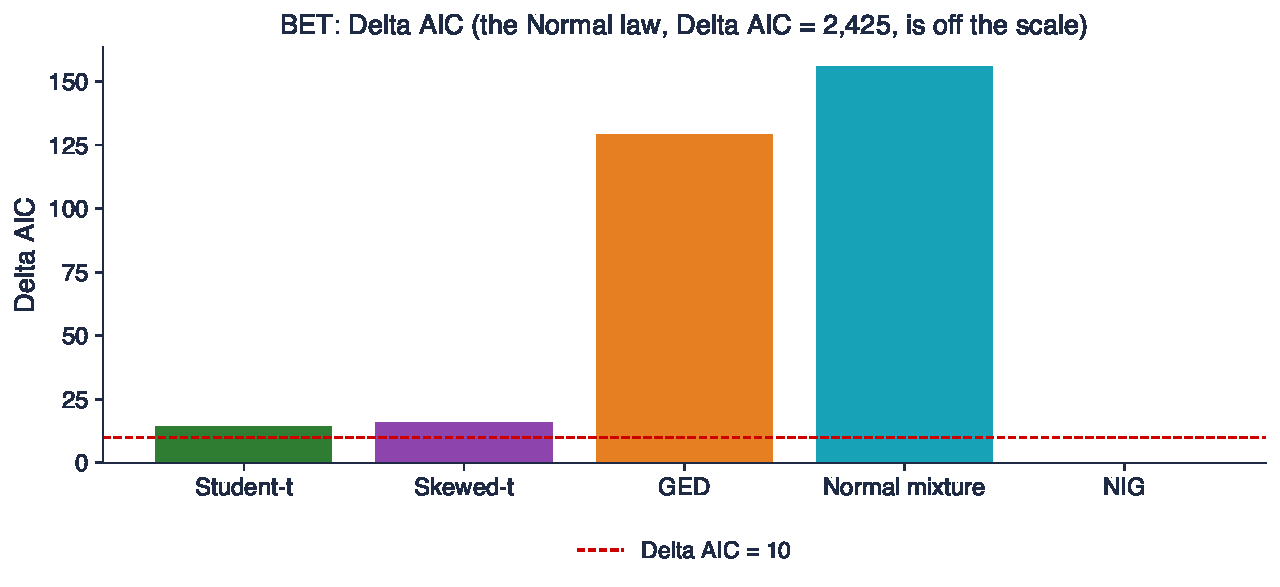
\includegraphics[width=0.96\textwidth,height=0.30\textheight,keepaspectratio]{ch6_sem_b1.pdf}
\end{center}
\vspace{-2mm}
\begin{center}
\tiny
\begin{tabular}{lrrrrrr}
\toprule
& $\ell(\hat\theta)$ & AIC & BIC & $\Delta$AIC & $\Delta$BIC & $w$ \\
\midrule
Normal & $-11\,702$ & $23\,407$ & $23\,421$ & $2425.2$ & $2411.6$ & $0.000$ \\
Student-t & $-10\,495$ & $20\,996$ & $21\,017$ & $14.4$ & $7.6$ & $0.001$ \\
skewed-t & $-10\,495$ & $20\,998$ & $21\,025$ & $16.0$ & $16.0$ & $0.000$ \\
GED & $-10\,553$ & $21\,111$ & $21\,132$ & $129.1$ & $122.3$ & $0.000$ \\
Normal mixture & $-10\,564$ & $21\,138$ & $21\,172$ & $155.8$ & $162.7$ & $0.000$ \\
NIG & $-10\,487$ & $20\,982$ & $21\,009$ & $0.0$ & $0.0$ & $0.999$ \\
\bottomrule
\end{tabular}
\end{center}
\begin{itemize}
    \item Winner: NIG on both criteria; Student-t $\hat\nu = 2.43$; skewed-t $\hat\lambda = -0.009$; $LR = 0.35$, $p = 0.555$: skewness not needed
    \item Interpretation: very heavy tails ($\nu$ close to 2) and no significant skewness; the Normal law is off by thousands of AIC points
\end{itemize}\quantlet{SFM\_ch6\_seminar}{\qlurl{SFM_ch6_seminar}}
\end{frame}

\begin{frame}{B2: DAX and Bitcoin [Proposed]}
\itemsize{\footnotesize}
\begin{itemize}
\item \textbf{Question}: do the DAX and Bitcoin choose the same distribution as the BET? Model: B1.
\item \textbf{Inputs}: DAX since 2000, Bitcoin since 2014 (7 days a week), daily log returns in \%
\item \textbf{Tasks}
\begin{enumerate}
    \item Repeat steps 1--3 of B1 for each series.
    \item Say whether AIC and BIC agree for each series.
    \item Interpretation: why might the best model differ between a stock index and a crypto asset?
\end{enumerate}
\item \textbf{Report}: two tables and three sentences
\item Notebook: section B2
\end{itemize}
\end{frame}

\ifsolutions
\begin{frame}{B2: Solution [Proposed]}
\itemsize{\footnotesize}
\begin{center}
\scriptsize
\begin{tabular}{lrrrrrr}
\toprule
& DAX $\Delta$AIC & DAX $\Delta$BIC & DAX $w$ & Bitcoin $\Delta$AIC & Bitcoin $\Delta$BIC & Bitcoin $w$ \\
\midrule
Normal & $1357.1$ & $1343.4$ & $0.000$ & $1429.5$ & $1423.1$ & $0.000$ \\
Student-t & $50.6$ & $43.8$ & $0.000$ & $94.6$ & $94.6$ & $0.000$ \\
skewed-t & $31.7$ & $31.7$ & $0.000$ & $96.1$ & $102.5$ & $0.000$ \\
GED & $44.8$ & $38.0$ & $0.000$ & $0.0$ & $0.0$ & $1.000$ \\
Normal mixture & $129.0$ & $135.8$ & $0.000$ & $158.6$ & $171.4$ & $0.000$ \\
NIG & $0.0$ & $0.0$ & $1.000$ & $28.5$ & $34.9$ & $0.000$ \\
\bottomrule
\end{tabular}
\end{center}
\begin{itemize}
    \item DAX: NIG (AIC and BIC); $LR$(Student-t vs skewed-t) $= 20.92$, $p <0.001$: skewness needed, $\hat\lambda = -0.070$
    \item Bitcoin: GED (AIC and BIC), GED $\hat\beta = 0.80$; $LR = 0.42$, $p = 0.515$: no skewness
    \item Interpretation: Bitcoin has a very sharp peak (many quiet days) and a different tail shape; the DAX has crash asymmetry, the BET does not
\end{itemize}\quantlet{SFM\_ch6\_seminar}{\qlurl{SFM_ch6_seminar}}
\end{frame}
\fi

\begin{frame}{B3: Do the Best Models Pass? [Solved]}
\itemsize{\footnotesize}
\begin{itemize}
\item \textbf{Question}: do the Normal and Student-t fits of the S\&P 500 pass the KS, Cramér--von Mises and Anderson--Darling tests?
\item \textbf{Inputs}: S\&P 500 daily log returns since 2000 ($n = 6\,714$)
\item \textbf{Tasks}
\begin{enumerate}
    \item Fit both models and compute the three statistics.
    \item Compute the naive KS $p$-value, which treats the parameters as known.
    \item Compute parametric bootstrap $p$-values with $B = 99$ (simulate, refit, recompute).
    \item Draw the QQ plot of the data against both fits.
    \item Interpretation: if both models are rejected, what is the test still good for?
\end{enumerate}
\item \textbf{Report}: a table of six statistics with $p$-values, the QQ plot and two sentences
\item Notebook: section B3
\end{itemize}
\end{frame}

\begin{frame}{B3: Solution [Solved]}
\itemsize{\scriptsize}
\begin{center}
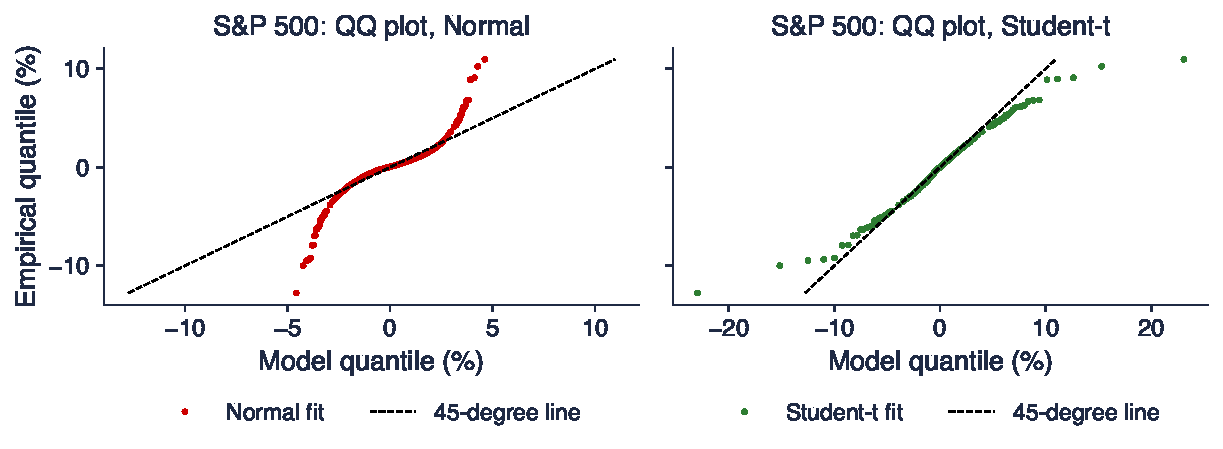
\includegraphics[width=0.96\textwidth,height=0.34\textheight,keepaspectratio]{ch6_sem_b3.pdf}
\end{center}
\vspace{-2mm}
\begin{center}
\tiny
\begin{tabular}{lrrrr}
\toprule
& KS & CvM & AD & KS naive $p$ \\
\midrule
Normal & $0.093$ & $22.84$ & $127.35$ & $<0.001$ \\
bootstrap 95\% critical value & $0.011$ & $0.12$ & $0.75$ &  \\
Student-t & $0.018$ & $0.57$ & $4.69$ & $0.021$ \\
bootstrap 95\% critical value & $0.009$ & $0.08$ & $0.65$ &  \\
\bottomrule
\end{tabular}
\end{center}
\begin{itemize}
    \item Bootstrap $p = 0.01$ for every statistic and both models (the smallest possible with $B = 99$): both rejected; the naive KS $p$ of the Student-t is far too large
    \item Interpretation: with $n = 6\,714$ any i.i.d.\ model is rejected; the statistics still rank the models (Student-t AD $4.69$ vs $127.35$), and the QQ plot shows where each fails
\end{itemize}\quantlet{SFM\_ch6\_seminar}{\qlurl{SFM_ch6_seminar}}
\end{frame}

\begin{frame}{B4: Crash or Data Error? Banca Transilvania [Proposed]}
\itemsize{\scriptsize}
\begin{itemize}
\item \textbf{Question}: which of the largest TLV returns are real, and does removing the wrong ones change the chosen model? Model: B1.
\item \textbf{Inputs}: TLV adjusted close since 2010, daily log returns in \%; the close (not adjusted) for comparison; the BET on the same days
\item \textbf{Tasks}
\begin{enumerate}
    \item List the three largest absolute returns with their dates.
    \item For each, compare the close and the adjusted close around the date, and the BET return of the same day.
    \item Decide which days are data errors and remove only those.
    \item Refit five candidates; compare the kurtosis, the Student-t $\hat\nu$, the AD statistic and the AIC winner before and after.
    \item Interpretation: what would have happened if you had removed all three days?
\end{enumerate}
\item \textbf{Report}: a table of three days with your verdict, a before/after table and two sentences
\item Notebook: section B4
\end{itemize}
\end{frame}

\ifsolutions
\begin{frame}{B4: Solution [Proposed]}
\itemsize{\scriptsize}
\begin{itemize}
    \item Largest absolute returns: 2016-05-30 ($-15.0\%$), 2016-05-31 ($20.5\%$), 2018-12-19 ($-22.2\%$)
    \begin{itemize}
        \item 30 May 2016: the close falls from $2.83$ to $2.09$ (bonus shares), the adjusted close only from $3.60$ to $3.10$, then jumps to $3.81$: the adjustment is one day late, \textbf{data error}
        \item 19 December 2018: close and adjusted close both fall about $20\%$, the BET falls $-11.9\%$ the same day (the bank tax announced in December 2018): a \textbf{real crash}, keep it
    \end{itemize}
    \item Before $\to$ after removing the two May 2016 days
    \begin{itemize}
        \item kurtosis $20.5 \to 16.5$; standard deviation $1.805 \to 1.758$; Student-t $\hat\nu$ $3.33 \to 3.44$; AD $1.29 \to 1.30$; AIC winner Student-t $\to$ Student-t
    \end{itemize}
    \item Interpretation: removing the real crash too would hide the risk the model is built for; clean only proven errors
\end{itemize}\quantlet{SFM\_ch6\_seminar}{\qlurl{SFM_ch6_seminar}}
\end{frame}
\fi

\begin{frame}{B5: VaR 1\% Out of Sample for the DAX [Solved]}
\itemsize{\scriptsize}
\begin{itemize}
\item \textbf{Question}: does the model chosen by AIC on 2000--2019 also give the best VaR 1\% on 2020--2026?
\item \textbf{Inputs}: DAX daily log returns: estimation 2000--2019 ($n = 5\,075$), test 2020--2026 ($n = 1\,710$)
\item \textbf{Tasks}
\begin{enumerate}
    \item Fit the six candidates on the estimation days and rank them by AIC.
    \item Compute each model's mean log score on the test days.
    \item Compute each model's VaR 1\%, count its exceedances on the test days and run the Kupiec test.
    \item Add historical simulation (the 1\% quantile of the estimation days) and the VaR averaged with the Akaike weights.
    \item Interpretation: which model would you choose for VaR 1\%, and why?
\end{enumerate}
\item \textbf{Report}: one table, the chart and two sentences
\item Notebook: section B5
\end{itemize}
\end{frame}

\begin{frame}{B5: Solution [Solved]}
\itemsize{\scriptsize}
\begin{center}
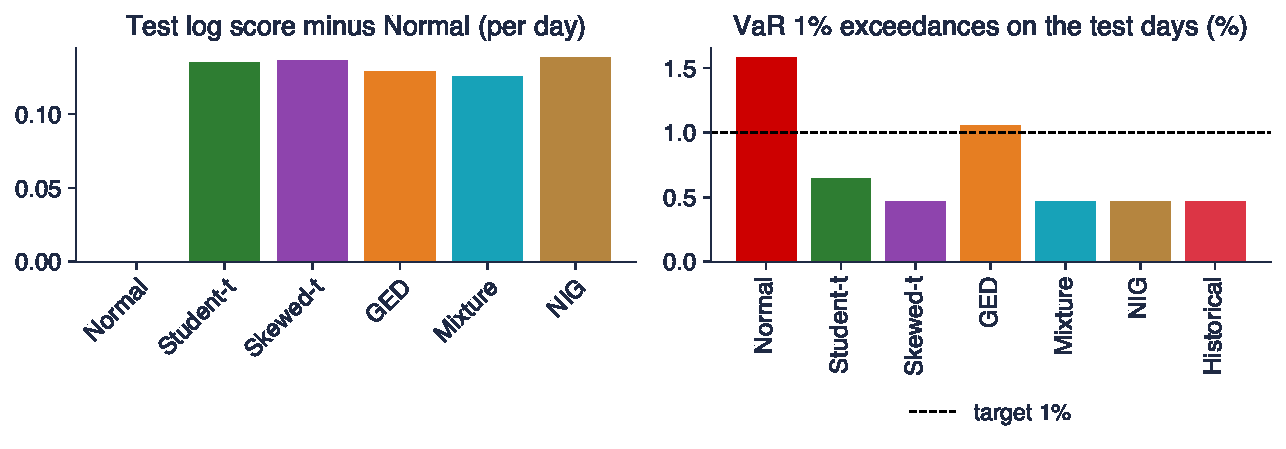
\includegraphics[width=0.96\textwidth,height=0.28\textheight,keepaspectratio]{ch6_sem_b5.pdf}
\end{center}
\vspace{-2mm}
\begin{center}
\tiny
\begin{tabular}{lrrrrr}
\toprule
& log score & VaR 1\% & exceed. & Kupiec $p$ & pinball $\times 100$ \\
\midrule
Normal & $-1.668$ & $3.37$ & 27 & $0.027$ & $5.37$ \\
Student-t & $-1.533$ & $4.09$ & 11 & $0.113$ & $5.23$ \\
skewed-t & $-1.532$ & $4.38$ & 8 & $0.014$ & $5.36$ \\
GED & $-1.539$ & $3.91$ & 18 & $0.828$ & $5.21$ \\
Normal mixture & $-1.542$ & $4.39$ & 8 & $0.014$ & $5.37$ \\
NIG & $-1.530$ & $4.38$ & 8 & $0.014$ & $5.36$ \\
historical & -- & $4.33$ & 8 & $0.014$ & $5.33$ \\
averaged & -- & $4.37$ & 8 & $0.014$ & $5.36$ \\
\bottomrule
\end{tabular}
\end{center}
\begin{itemize}
    \item AIC on 2000--2019: NIG; best test log score: NIG; expected exceedances 17.1; lowest pinball loss: GED
    \item Interpretation: the AIC winner gives the best density but too few exceedances (too prudent); for VaR 1\% alone the GED and the Student-t were closer to 1\%
\end{itemize}\quantlet{SFM\_ch6\_seminar}{\qlurl{SFM_ch6_seminar}}
\end{frame}

\begin{frame}{B6: VaR 1\% Out of Sample for Bitcoin [Proposed]}
\itemsize{\footnotesize}
\begin{itemize}
\item \textbf{Question}: does the B5 conclusion hold for Bitcoin? Model: B5.
\item \textbf{Inputs}: Bitcoin: estimation 2014--2019 ($n = 1\,931$), test 2020--2026 ($n = 2\,453$)
\item \textbf{Tasks}
\begin{enumerate}
    \item Repeat steps 1--4 of B5.
    \item Compare the empirical VaR 1\% of the test days with that of the estimation days.
    \item Interpretation: why do all heavy-tailed models fail the Kupiec test here, and in which direction?
\end{enumerate}
\item \textbf{Report}: one table and two sentences
\item Notebook: section B6
\end{itemize}
\end{frame}

\ifsolutions
\begin{frame}{B6: Solution [Proposed]}
\itemsize{\footnotesize}
\begin{center}
\scriptsize
\begin{tabular}{lrrrrr}
\toprule
& log score & VaR 1\% & exceed. & Kupiec $p$ & pinball $\times 100$ \\
\midrule
Normal & $-2.605$ & $8.83$ & 23 & $0.754$ & $12.97$ \\
Student-t & $-2.443$ & $13.48$ & 7 & $<0.001$ & $15.36$ \\
skewed-t & $-2.443$ & $13.32$ & 7 & $<0.001$ & $15.24$ \\
GED & $-2.443$ & $11.33$ & 10 & $<0.001$ & $13.87$ \\
Normal mixture & $-2.462$ & $11.32$ & 10 & $<0.001$ & $13.87$ \\
NIG & $-2.438$ & $12.56$ & 7 & $<0.001$ & $14.70$ \\
historical & -- & $11.39$ & 10 & $<0.001$ & $13.91$ \\
averaged & -- & $11.33$ & 10 & $<0.001$ & $13.87$ \\
\bottomrule
\end{tabular}
\end{center}
\begin{itemize}
    \item Expected exceedances 24.5; best test log score: NIG; lowest pinball loss: Normal
    \item Empirical VaR 1\% of the test days: $8.63\%$, against $11.39\%$ on the estimation days: Bitcoin became calmer
    \item Interpretation: all heavy-tailed models are too prudent (too few exceedances); the Normal model passes by accident: a static model fitted on a turbulent past cannot follow a calmer present
\end{itemize}\quantlet{SFM\_ch6\_seminar}{\qlurl{SFM_ch6_seminar}}
\end{frame}
\fi


%=============================================================================
\section{Part C: Open Questions and AI Critique}
%=============================================================================

\begin{frame}{C1: Does the Best Model Change over Time? [Proposed]}
\itemsize{\footnotesize}
\begin{itemize}
\item \textbf{Question}: is the AIC winner of the S\&P 500 and the BET the same in every two-year window?
\item \textbf{Inputs}: daily log returns since 2000, non-overlapping two-year windows (2000--2001, 2002--2003, ...); candidates: Normal, Student-t, skewed-t, GED, NIG; models: B1, A1
\item \textbf{Tasks}
\begin{enumerate}
    \item In each window, find the AIC winner, its Akaike weight and the $\Delta$AIC of the runner-up.
    \item Count how often each model wins, for each index.
    \item Propose one explanation for the changes and one way to test it.
    \item Interpretation: should a risk model be re-selected every two years?
\end{enumerate}
\item \textbf{Report}: a table, a count of winners and a plan for a project
\item Notebook: section C1
\end{itemize}
\end{frame}

\ifsolutions
\begin{frame}{C1: Reference Analysis [Proposed]}
\itemsize{\scriptsize}
\begin{columns}[T]
\begin{column}{0.48\textwidth}
\centering S\&P 500\begin{center}
\tiny
\begin{tabular}{llrlr}
\toprule
window & winner & $w$ & runner-up & $\Delta$ \\
\midrule
2000--2001 & Student-t & $0.46$ & NIG & $1.7$ \\
2002--2003 & GED & $0.44$ & Student-t & $1.0$ \\
2004--2005 & Normal & $0.41$ & skewed-t & $1.5$ \\
2006--2007 & GED & $0.81$ & NIG & $3.0$ \\
2008--2009 & GED & $0.50$ & NIG & $0.3$ \\
2010--2011 & GED & $0.92$ & NIG & $5.1$ \\
2012--2013 & GED & $0.68$ & NIG & $3.0$ \\
2014--2015 & GED & $0.90$ & NIG & $5.1$ \\
2016--2017 & GED & $0.75$ & NIG & $2.3$ \\
2018--2019 & NIG & $0.83$ & GED & $4.1$ \\
2020--2021 & skewed-t & $0.48$ & Student-t & $0.2$ \\
2022--2023 & GED & $0.69$ & Student-t & $3.0$ \\
2024--2025 & skewed-t & $0.73$ & Student-t & $2.5$ \\
\bottomrule
\end{tabular}
\end{center}

\end{column}
\begin{column}{0.48\textwidth}
\centering BET\begin{center}
\tiny
\begin{tabular}{llrlr}
\toprule
window & winner & $w$ & runner-up & $\Delta$ \\
\midrule
2000--2001 & Student-t & $0.39$ & skewed-t & $0.3$ \\
2002--2003 & NIG & $0.83$ & GED & $3.9$ \\
2004--2005 & Student-t & $0.59$ & skewed-t & $1.6$ \\
2006--2007 & GED & $0.59$ & Student-t & $2.7$ \\
2008--2009 & NIG & $0.37$ & Student-t & $0.5$ \\
2010--2011 & Student-t & $0.71$ & skewed-t & $2.0$ \\
2012--2013 & Student-t & $0.66$ & skewed-t & $2.0$ \\
2014--2015 & Student-t & $0.68$ & skewed-t & $2.0$ \\
2016--2017 & Student-t & $0.65$ & skewed-t & $1.8$ \\
2018--2019 & Student-t & $0.67$ & skewed-t & $1.4$ \\
2020--2021 & Student-t & $0.53$ & skewed-t & $0.7$ \\
2022--2023 & skewed-t & $0.43$ & NIG & $0.4$ \\
2024--2025 & skewed-t & $0.52$ & NIG & $0.5$ \\
\bottomrule
\end{tabular}
\end{center}

\end{column}
\end{columns}\begin{itemize}
    \item S\&P 500: GED wins 8 of 13 windows; BET: Student-t wins 8 of 13; the runner-up is often within $\Delta < 2$
    \item The full-sample winner (NIG) rarely wins in short windows: with $n \approx 500$ the candidates are hard to separate, and volatility regimes change the shape
    \item Project directions: standardise by a volatility model first; longer windows; more markets
\end{itemize}\quantlet{SFM\_ch6\_seminar}{\qlurl{SFM_ch6_seminar}}
\end{frame}
\fi

\begin{frame}{C2: Audit an AI Answer [Proposed]}
\itemsize{\scriptsize}
\begin{itemize}
    \item A student asked an AI assistant to choose a distribution for the daily S\&P 500 log returns (\%) since 2000 ($n = 6\,714$). The answer:
    \item \aiprompt{(a) The skewed-t has the lowest AIC, so it is significantly better than the Student-t (Delta AIC = 17.6).}
    \item \aiprompt{(b) The KS test of the Student-t fit gives p = 0.021 with scipy.stats.kstest, so the Student-t fits at the 1\% level.}
    \item \aiprompt{(c) The LR test of Normal vs Student-t uses the chi2(1) critical value 3.84.}
    \item \aiprompt{(d) BIC penalises extra parameters less than AIC, because ln(n) is only 8.81.}
    \item \aiprompt{(e) The Anderson-Darling test is more sensitive than KS to the fit in the tails.}
    \item \aiprompt{(f) Since the skewed-t has the best fit, its VaR 1\% is the most accurate one.}
    \item Tasks
    \begin{itemize}
        \item 1. For each statement, say whether it is correct; if not, give the correct statement and, where possible, the correct number from the notebook (section C2).
        \item 2. Report: a list of six verdicts with one line of justification each.
    \end{itemize}
\end{itemize}
\end{frame}

\ifsolutions
\begin{frame}{C2: Solution [Proposed]}
\itemsize{\footnotesize}
\begin{itemize}
    \item (a) Wrong wording: AIC is not a test and has no ``significance''; a $\Delta$AIC of $17.6$ is strong evidence by the rules of thumb (the LR test of $\lambda = 0$ agrees)
    \item (b) Wrong: the parameters were estimated on the same data, so the naive KS $p$ is too large; a parametric bootstrap gives $p \le 0.01$, and $p = 0.021 < 0.05$ anyway
    \item (c) Wrong: $1/\nu = 0$ lies on the boundary; the correct 5\% critical value is $2.71$ (the decision does not change: $LR = 1\,949$)
    \item (d) Wrong: $\ln n = 8.81 > 2$, so BIC penalises each parameter more than four times as much as AIC
    \item (e) Correct: AD weights the squared gap by $1/[F(1 - F)]$, large in the tails
    \item (f) Wrong logic: the best overall fit does not imply the best quantile; in sample the skewed-t VaR 1\% is $3.71\%$, the Student-t $3.46\%$, the data $3.45\%$; judge VaR by its exceedances out of sample
\end{itemize}\quantlet{SFM\_ch6\_seminar}{\qlurl{SFM_ch6_seminar}}
\end{frame}
\fi


%=============================================================================
\section{Wrap-Up}
%=============================================================================

\begin{frame}{What You Should Take from Today}
\itemsize{\small}
\begin{itemize}
    \item AIC and BIC rank models; $\Delta \le 2$ is a tie; Akaike weights turn $\Delta$ into evidence
    \item LR tests need nested models and a parameter inside the space; on the boundary use the 50:50 mixture
    \item KS with estimated parameters needs Lilliefors or a bootstrap; AD sees the tails, KS does not
    \item Check the largest returns before modelling: remove errors, keep crashes
    \item The best density is not always the best VaR: validate out of sample
\end{itemize}
\end{frame}

\begin{frame}{After the Seminar}
\itemsize{\small}
\begin{itemize}
    \item Lecture 6 develops each topic of today: likelihood, LR and Vuong tests, AIC and BIC, EDF tests, QQ plots, out-of-sample VaR, model uncertainty
    \item Try the [Proposed] tasks in the notebook; the solutions are discussed in class
    \item C1 can grow into a team project: standardised returns, more markets, rolling windows
    \item Reading: \refBA; \refStephens; \refKupiec
\end{itemize}
\end{frame}


%=============================================================================
\section{References}
%=============================================================================

\begin{frame}{References}
\itemsize{\tiny}
\begin{itemize}
    \item Akaike, H. (1974). \href{https://doi.org/10.1109/TAC.1974.1100705}{A new look at the statistical model identification}. \textit{IEEE Transactions on Automatic Control}, 19(6), 716--723.
    \item Burnham, K.P., Anderson, D.R. (2004). \href{https://doi.org/10.1177/0049124104268644}{Multimodel inference: understanding AIC and BIC in model selection}. \textit{Sociological Methods \& Research}, 33(2), 261--304.
    \item Franke, J., Härdle, W.K., Hafner, C.M. (2019). \href{https://doi.org/10.1007/978-3-030-13751-9}{\textit{Statistics of Financial Markets: An Introduction}}, 5th ed. Springer.
    \item Hansen, B.E. (1994). \href{https://doi.org/10.2307/2527081}{Autoregressive conditional density estimation}. \textit{International Economic Review}, 35(3), 705--730.
    \item Kupiec, P.H. (1995). \href{https://doi.org/10.3905/jod.1995.407942}{Techniques for verifying the accuracy of risk measurement models}. \textit{Journal of Derivatives}, 3(2), 73--84.
    \item Lilliefors, H.W. (1967). \href{https://doi.org/10.1080/01621459.1967.10482916}{On the Kolmogorov--Smirnov test for normality with mean and variance unknown}. \textit{Journal of the American Statistical Association}, 62(318), 399--402.
    \item Schwarz, G. (1978). \href{https://doi.org/10.1214/aos/1176344136}{Estimating the dimension of a model}. \textit{Annals of Statistics}, 6(2), 461--464.
    \item Self, S.G., Liang, K.-Y. (1987). \href{https://doi.org/10.1080/01621459.1987.10478472}{Asymptotic properties of maximum likelihood estimators and likelihood ratio tests under nonstandard conditions}. \textit{Journal of the American Statistical Association}, 82(398), 605--610.
    \item Stephens, M.A. (1974). \href{https://doi.org/10.1080/01621459.1974.10480196}{EDF statistics for goodness of fit and some comparisons}. \textit{Journal of the American Statistical Association}, 69(347), 730--737.
    \item Wilks, S.S. (1938). \href{https://doi.org/10.1214/aoms/1177732360}{The large-sample distribution of the likelihood ratio for testing composite hypotheses}. \textit{Annals of Mathematical Statistics}, 9(1), 60--62.
\end{itemize}
\end{frame}

\end{document}
